\section{Propulsion}

\subsection{Overview}

To accelerate our Hyperloopod we use our EMRAX 188 electric motor from last season. This delivers an output of 60 kW under high voltage and a maximum torque of 100 Nm. This torque gets transferred to a right-angle gearbox and from there is slid to the drive wheels via cardan joints.

\subsubsection{Concept}
The main goal of this system is to accelerate our pod with an acceleration of \(5 \, \text{m/s}^2\). Since the given \(100 \, \text{Nm}\) are not sufficient under an estimated total weight of \(250 \, \text{kg}\), the drivetrain requires a gear ratio. Since an angular gearbox is installed anyway, it is easy to implement this criterion there. In order to maintain a relatively high top speed of the pod, this transmission ratio should be as close as possible. According to the formula
\[
T_{\text{required}} = \frac{{(m \cdot a + \frac{1}{2} \cdot \rho_{\text{air}} \cdot C_w \cdot A_{\text{Aeroshell}} \cdot v^2 + m \cdot g \cdot \cos(\Theta)) \cdot r}}{{\eta}}
\]
we know that we require at least around \(170 \, \text{Nm}\) of torque to achieve this amount of acceleration. While the pod weight of \(250 \, \text{kg}\) is only an estimate at the time of system design and we are always keen to get such complex parts from our partners, we opted for a \(2:1\) ratio of a Mädler gearbox. With this gear ratio, a respectable top speed of \(113 \, \text{km/h}\) is still possible. This is absolutely sufficient for our prototype, as we are still sticking to our basic idea: For low speeds and accelerations, we drive our hyperloop pod with a conventional wheel drive and for everything above that, the pod will hover with a linear induction motor which will be added in future prototypes. We believe that we can achieve an increase in efficiency in this way as permanent levitation is not necessary.

The transmitted torque must now be directed to the drive wheels in such a way that it is still possible to ensure a working suspension. For this, we use universal joints on both sides of the centered bevel gear. These also come from our partner Mädler and are connected to the bevel gear using in-house produced adapter shafts and feather keys. To finally connect the other ends of the shaft joints to the wheel, only one last shaft is missing. This is also fitted with a keyway on the joint side and a bolt circle on a flange on the wheel side. Now that the wheels are supplied with power, it is important to create sufficient rolling friction. To achieve this, Continental provides us with a rubber coating for our wheels. \\
Of course, this all has to be mounted into the chassis. For this, we use three different types of brackets beside the knuckles, where the wheelshafts are mounted: one for the motor, one for the motorshaft and two of the same kind, which carry everything between the shaft joints.

\subsubsection{Size, Components, and Appearance}

\autoref{table:components}
\begin{table}[ht]
\centering
\begin{adjustbox}{width=\textwidth}
\begin{tabular}{|>{\bfseries}m{2.5cm}|m{1.4cm}|m{1.7cm}|m{2.9cm}|m{2.2cm}|}
\hline
Component & Number & Mass [kg] & Size [mm] &  In-house/ outsourced \\
\hline
Motor & x1 & 7 & \(188 \times 188 \times 112\) &   Bought \\
Motorshaft & x1 & 0.4 & \(170 \times 83\times 83\) &Outsourced \\
Resolver & x1 & 1 & - &  Bought \\
Inverter & x1 & 9 & \(400 \times 400 \times 100\) &  Outsourced \\
Bevelgear z=20 & x1 & 3 & \(10 \times 90\) &  Bought \\
Bevelgear z=40 & x1 & 9.6 & \(20 \times 30 \times 50\) &Bought \\
Gearshaft Pressfitted & x1 & 0.3 & \(103 \times 40 \times 40\) & Outsourced \\
Gearshaft bolted & x1 & 0.7 & \(106 \times 55 \times 55\) &Outsourced \\
Shaft Joint & x2 & 4.1 & \(30 \times 40 \times 60\) &  Bought \\
Wheelshaft & x2 & 0.7 & \(138 \times 100 \times 100\) &   Outsourced \\
Wheel & x2 & 1.7 & \(200 \times 200 \times 155\) &  Outsourced \\
\hline
\end{tabular}
\end{adjustbox}
\caption{Components}
\label{table:components}
\end{table}

\subsection{Design Process and Appearance}

\subsubsection{Motor}

\begin{figure}[H]
\centering
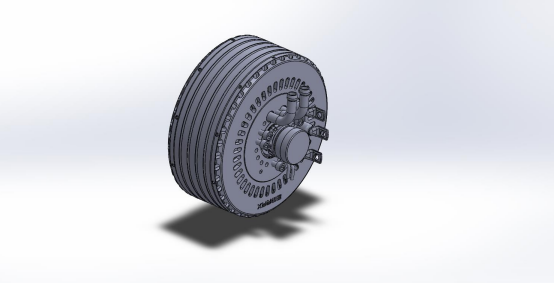
\includegraphics[width=0.6\textwidth]{texfiles/mech/eimg/propulsion/picture_motor}
\caption{CAD of EMRAX 188}
\label{}
\end{figure}

As previously mentioned, we are once again using our EMARX 188 electric motor from last season. You can find all the technical details in Table~\ref{tab: Motor Specifications} .



\subsubsection{Motorshaft}

\begin{figure}[ht!]
  \centering
  \begin{subfigure}{.5\textwidth}
    \centering
    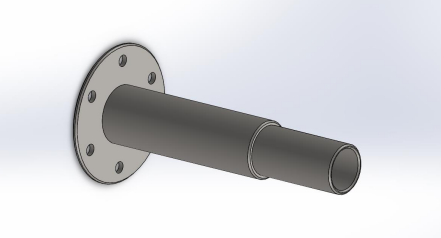
\includegraphics[width=\linewidth]{texfiles/mech/eimg/propulsion/picture_motorshaft}
    \caption{CAD Render}
    \label{fig:CAD Motorshaft}
  \end{subfigure}%
  \begin{subfigure}{.4\textwidth}
    \centering
    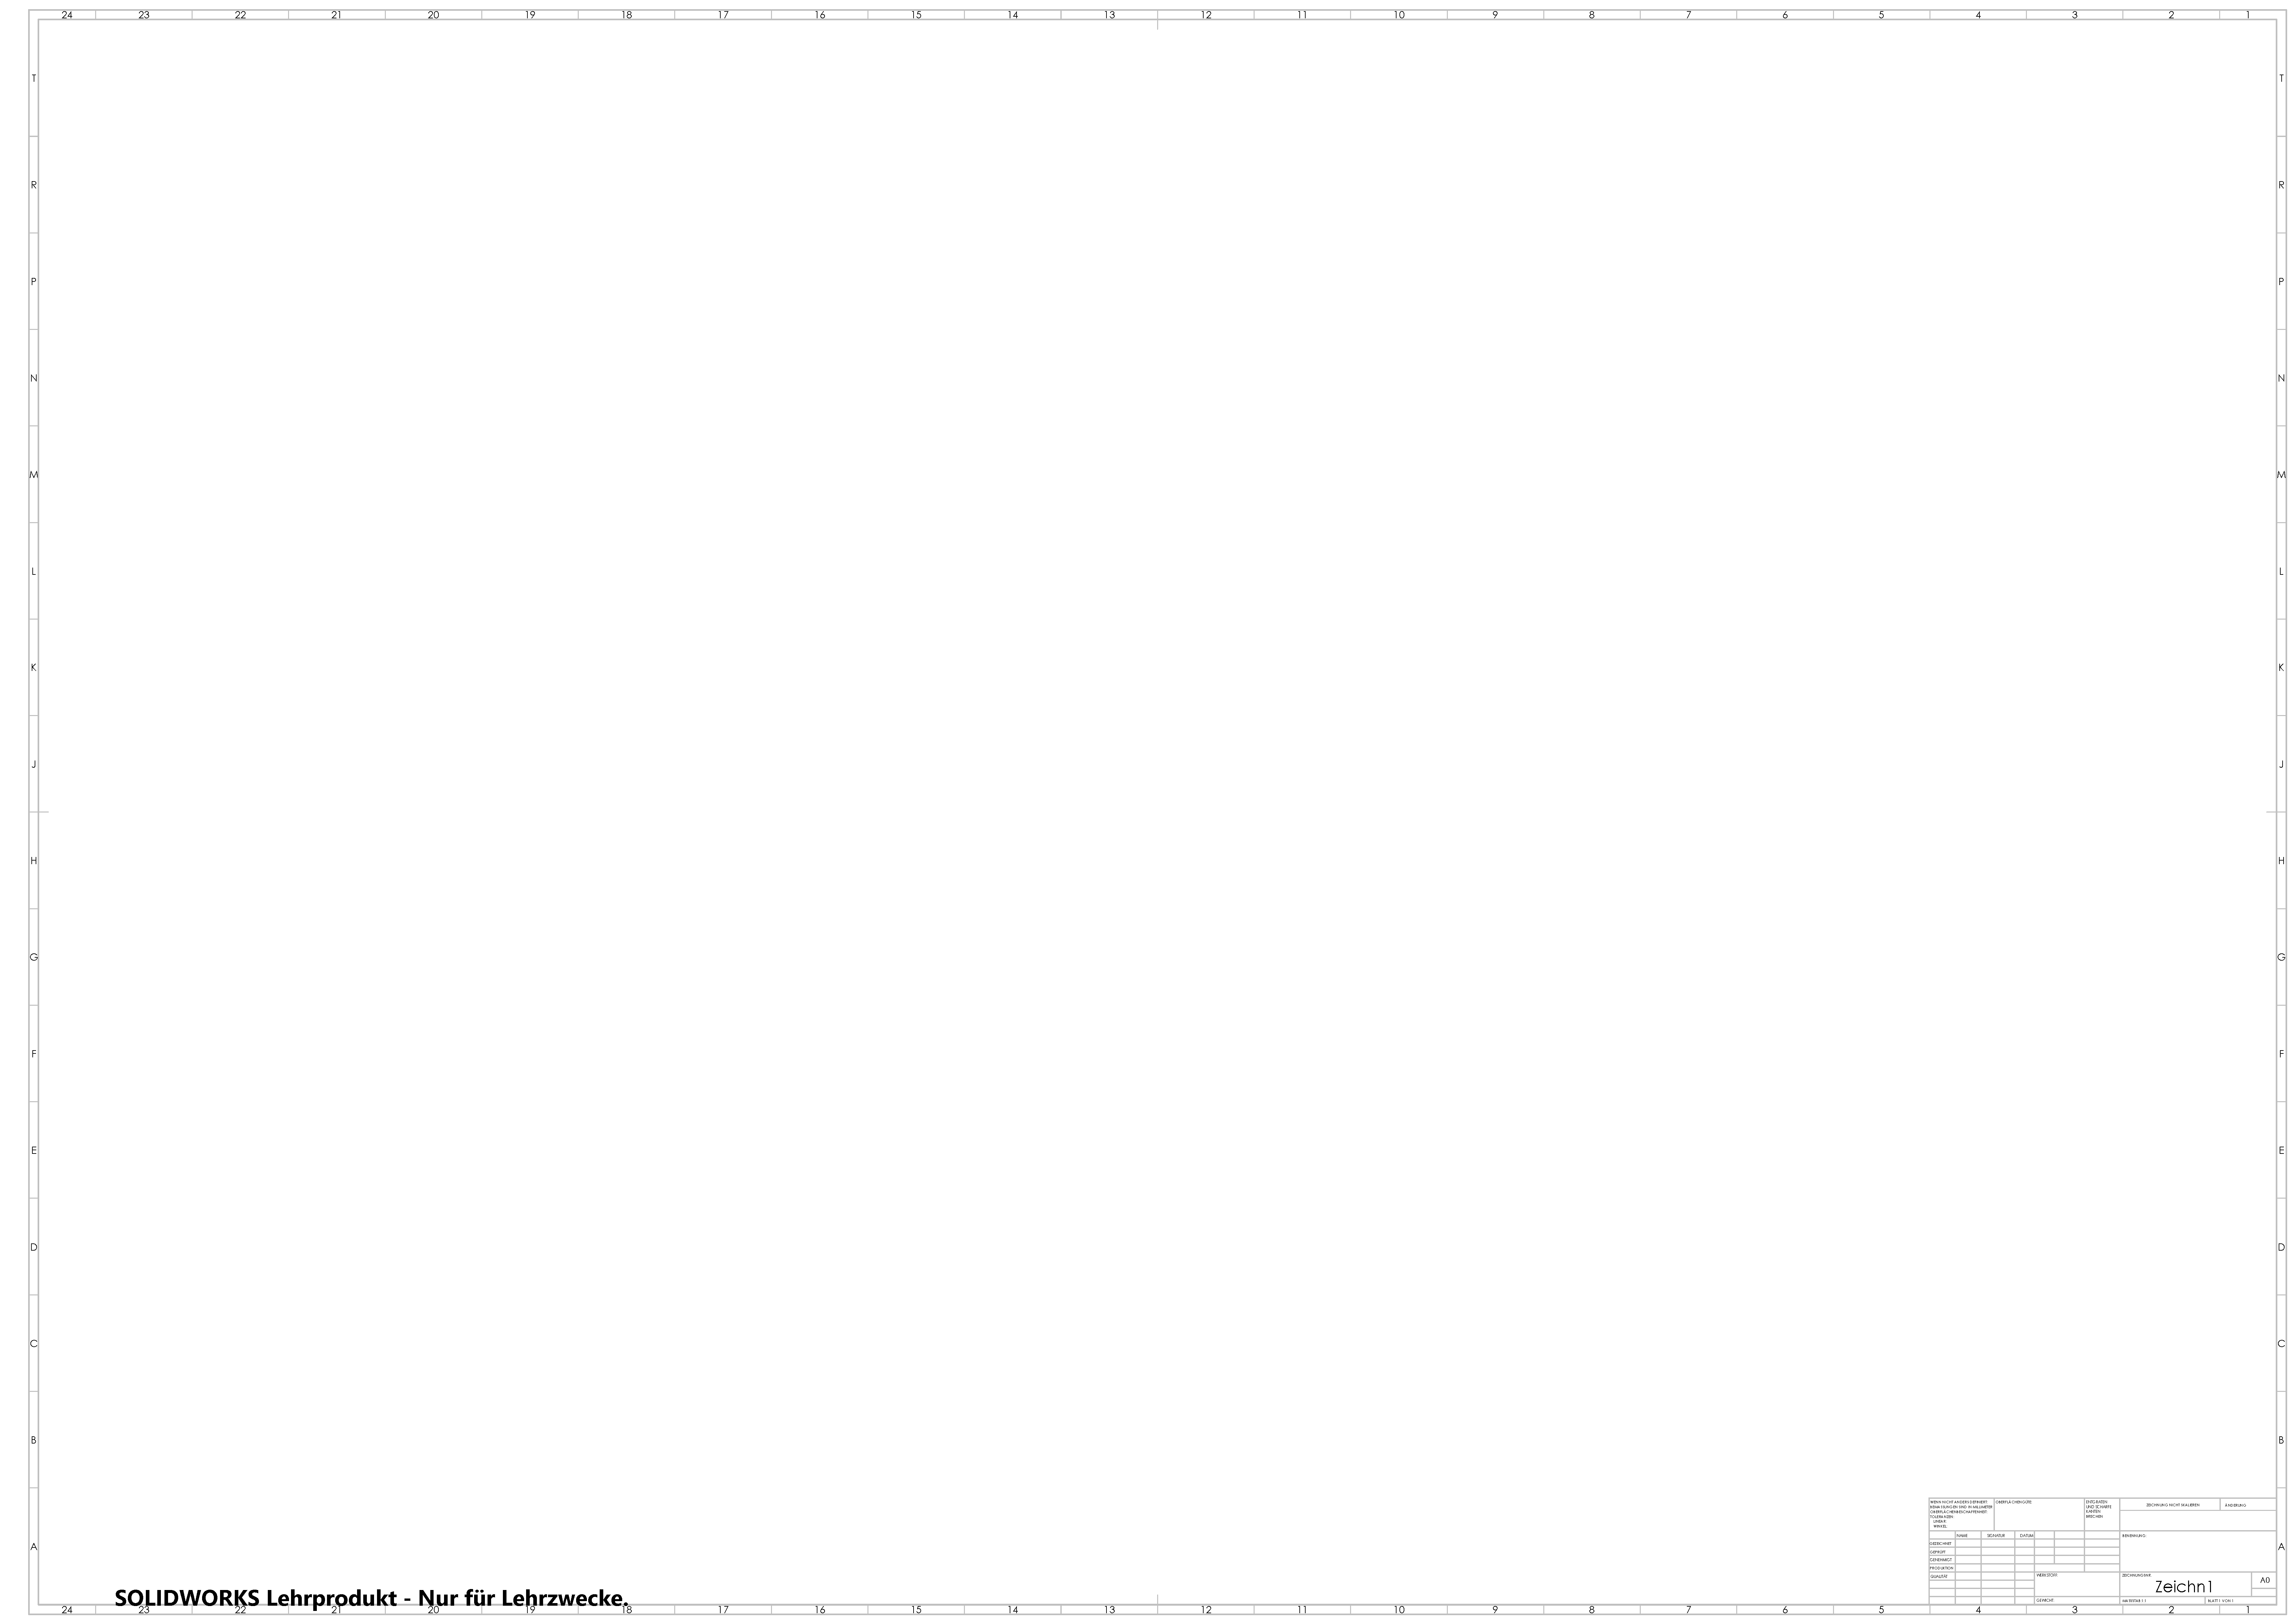
\includegraphics[width=\linewidth]{texfiles/mech/eimg/propulsion/spaceholder_technical_drawing}
    \caption{Technical Drawing}
    \label{fig:TD Motorshaft}
  \end{subfigure}
  \caption{Motor Bracket}
  \label{fig:Motorshaft}
\end{figure}



Even though it is a heavy material, C45 steel provides adequate tensile strength to transmit torque from the motor to the gearbox or from the gearbox to the wheels. To maintain a relatively low weight for this part, it is hollow like all the other shafts. In Figure \ref{fig:motorshaft_forces}, you can now see the applied forces. The shaft is mounted on the motor at the screw holes of the flange (green). This means that the motor torque of \(100 \, \text{Nm}\) (pink) acts up to the surface on which the bevel gear is pressed. The calculation of the contact pressure of \(16.26 \, \text{MPa}\) is given by
\[
p_{\text{contact}}=\frac{2\cdot M\cdot S_r}{\pi \cdot D^2 \cdot l\cdot \mu}
\]
In addition, there is a centrifugal force (blue) at maximum rotational speed of \(6000 \, \text{rpm}\).

\autoref{fig:motorshaft_forces}
\begin{figure}[H]
\centering
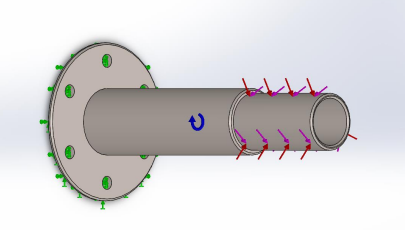
\includegraphics[width=0.6\textwidth]{texfiles/mech/eimg/propulsion/picture_forces_motorshaft}
\caption{Forces acting on the Motorshaft}
\label{fig:motorshaft_forces}
\end{figure}

\subsubsection{Bevel Gears}
picture gearbox

The bevel gears with the article numbers 36736000 and 36736100 are our choice to fulfill the desired purpose.
36736000 offers spur gearing with 20 teeth. With a maximum permissible torque of 130 Nm, it can withstand the prevailing forces. 
The larger counterpart 36736100 therefore has twice as many teeth (40 teeth) and is designed for a maximum torque of 260 Nm.

\subsubsection{Gearshafts}
\begin{figure}[H]
\centering
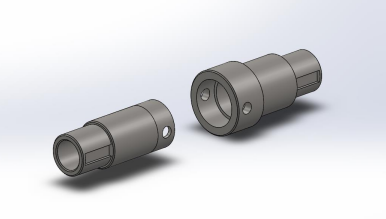
\includegraphics[width=0.6\textwidth]{texfiles/mech/eimg/propulsion/picture_gearshafts}
\caption{}
\label{}
\end{figure}

To be able to conduct the torque of the bevel gear, we have designed another shaft. This consists of two individual parts, one which is again pressed into the bevel gear and the other which is screwed onto the first part after pressing.
The specifications of the initially acting shaft are as follows:

\begin{figure}[ht!]
  \centering
  \begin{subfigure}{.5\textwidth}
    \centering
    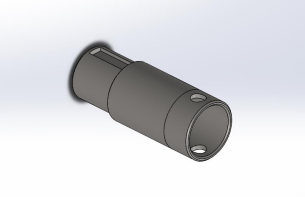
\includegraphics[width=\linewidth]{texfiles/mech/eimg/propulsion/picture_gearshaft_right}
    \caption{CAD Render}
    \label{fig:CAD Motorshaft}
  \end{subfigure}%
  \begin{subfigure}{.5\textwidth}
    \centering
    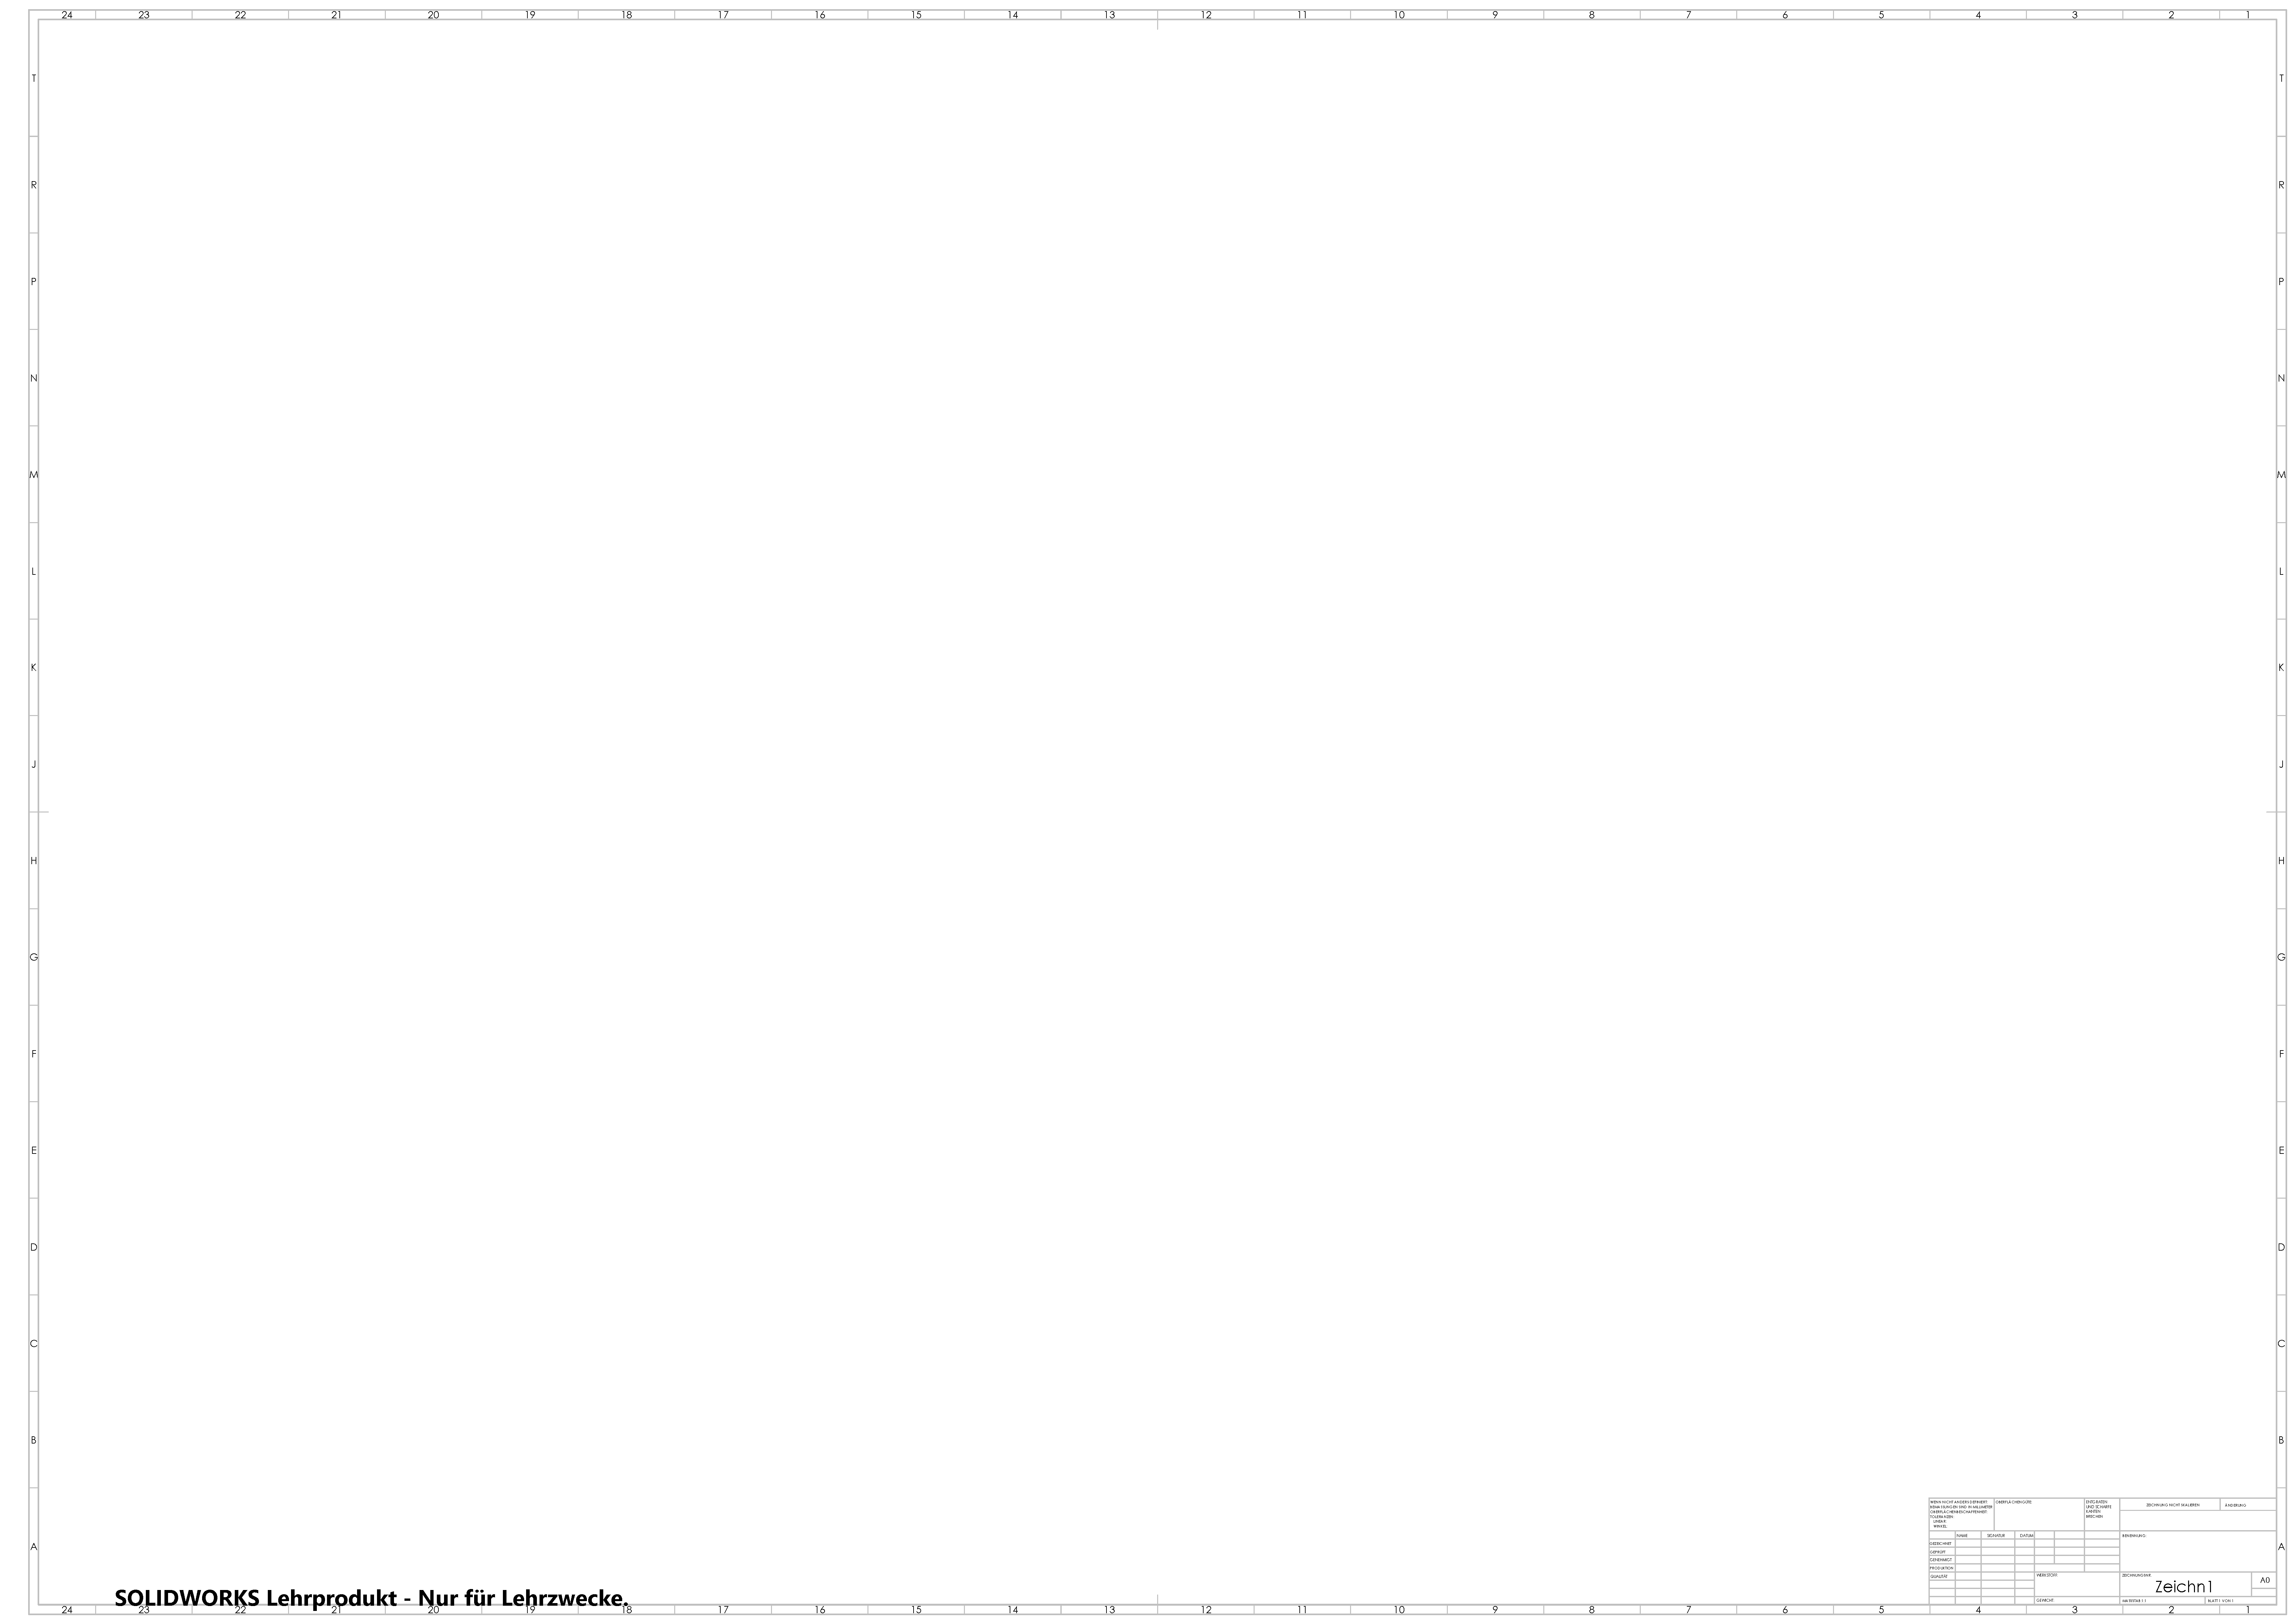
\includegraphics[width=\linewidth]{texfiles/mech/eimg/propulsion/spaceholder_technical_drawing}
    \caption{Technical Drawing}
    \label{fig:TD Motorshaft}
  \end{subfigure}
  \caption{Motor Bracket}
  \label{fig:Motorshaft}
  \end{figure}



Fig.xx  shows all the acting forces. For calculating the pressing force (red) we again use the formula for \(p_{\text{contact}}\)
and get the result of \(21.22 \, \text{MPa}\). The higher torque of \(200 \, \text{Nm}\) (pink) resulting from the gear ratio also acts on this surface and is transferred to the screw holes and keyway (green). A centrifugal force (blue) also acts on this part, but this has now been halved by the gear ratio and is therefore only based on \(3000 \, \text{rpm}\). Finally, we assume a bearing restraint (orange) at the shaft end to the shaft joint. The admissibility of this case is described in the paragraph on the shaft joint itself.

\begin{figure}[H]
\centering
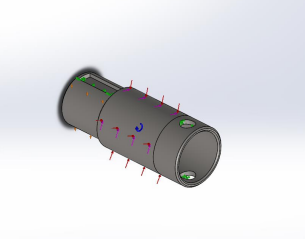
\includegraphics[width=0.6\textwidth]{texfiles/mech/eimg/propulsion/picture_forces_gearshaft_right}
\caption{Forces acting on the pressfitted Gearshaft}
\label{fig:gearshaft_right_forces}
\end{figure}


The torque is now transferred to the second part of the gearshaft:
\begin{figure}[ht!]
  \centering
  \begin{subfigure}{.5\textwidth}
    \centering
    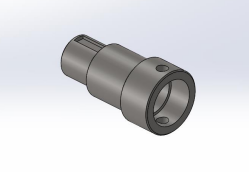
\includegraphics[width=\linewidth]{texfiles/mech/eimg/propulsion/picture_gearshaft_left}
    \caption{CAD Render}
    \label{fig:CAD Motorshaft}
  \end{subfigure}%
  \begin{subfigure}{.5\textwidth}
    \centering
    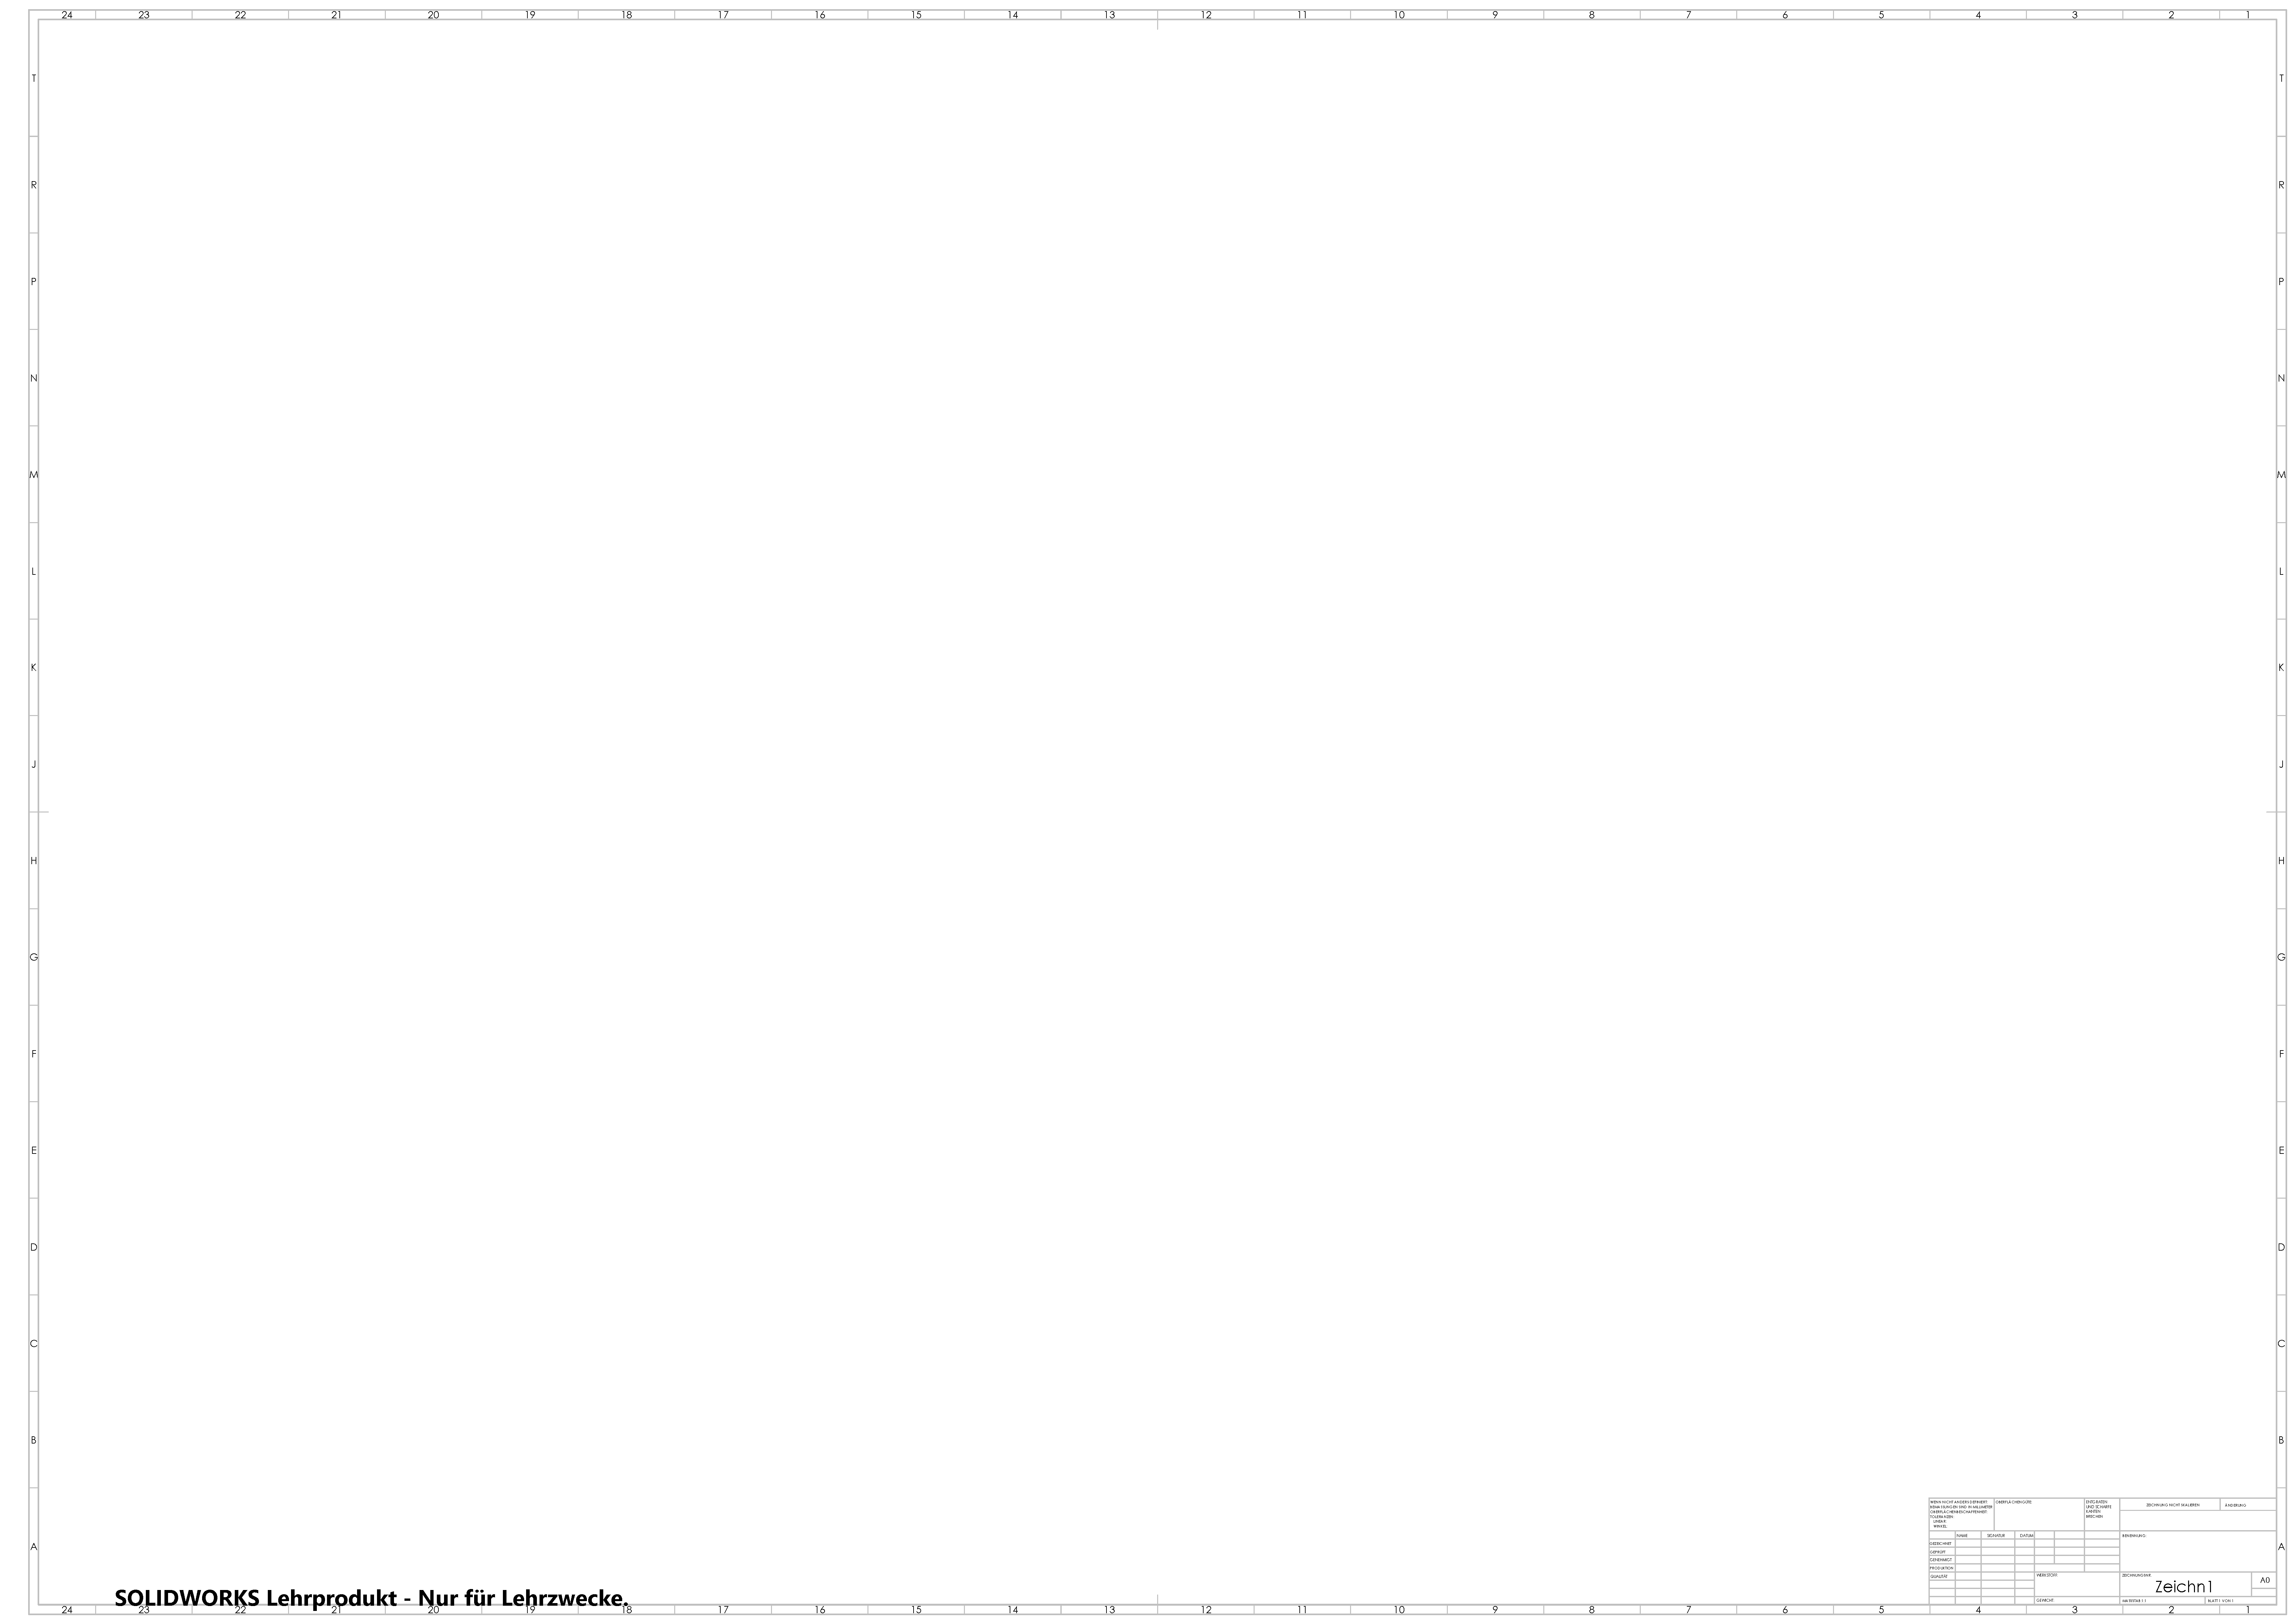
\includegraphics[width=\linewidth]{texfiles/mech/eimg/propulsion/spaceholder_technical_drawing}
    \caption{Technical Drawing}
    \label{fig:TD Motorshaft}
  \end{subfigure}
  \caption{Motor Bracket}
  \label{fig:Motorshaft}
  \end{figure}



Fig.xx shows all the forces acting on this part. The two shafts are connected to each other at the screw holes (green). The centrifugal force (blue) acts as in the first shaft at \(3000 \, \text{rpm}\) and the torque of \(200 \, \text{Nm}\) (pink) up to the keyway. This end piece of the shaft is also simulated as a bearing (orange).

\begin{figure}[H]
\centering
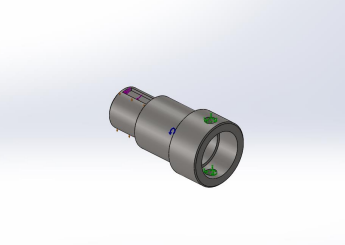
\includegraphics[width=0.6\textwidth]{texfiles/mech/eimg/propulsion/picture_forces_gearshaft_left}
\caption{Forces acting on the bolted Gearshaft}
\label{fig:gearshaft_left_forces}
\end{figure}

\subsubsection{Shaft Joints}
\begin{figure}[H]
\centering
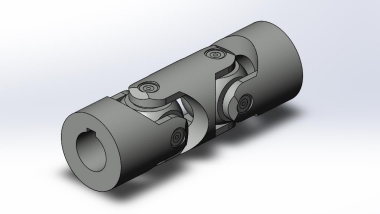
\includegraphics[width=0.6\textwidth]{texfiles/mech/eimg/propulsion/picture_shaft_joint}
\caption{}
\label{}
\end{figure}


To enable the system to absorb shocks, we use cardan shafts on each side. This allows the wheels to move vertically independently of the rest of the pod. Our partner Mädler is once again supplying us with such complex parts. Item number 63167000N is a double universal joint which we install in our system. It has a keyway at both ends and is designed to transmit 202 Nm at 3000 rpm. These specifications are almost perfect for our drive power.
We will mount the heart of our system at the ends of this joint adjacent to the gearbox. This is also the reason why a bearing is created at the respective ends in the simulations of the shafts because this bearing is also attached above the respective area.
However, more on the bearing and attachment points will follow in the corresponding sections.

\subsubsection{Wheelshafts}
\begin{figure}[ht!]
  \centering
  \begin{subfigure}{.5\textwidth}
    \centering
    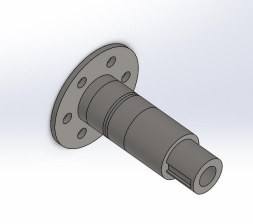
\includegraphics[width=\linewidth]{texfiles/mech/eimg/propulsion/picture_wheelshaft}
    \caption{CAD Render}
    \label{fig:CAD Motorshaft}
  \end{subfigure}%
  \begin{subfigure}{.5\textwidth}
    \centering
    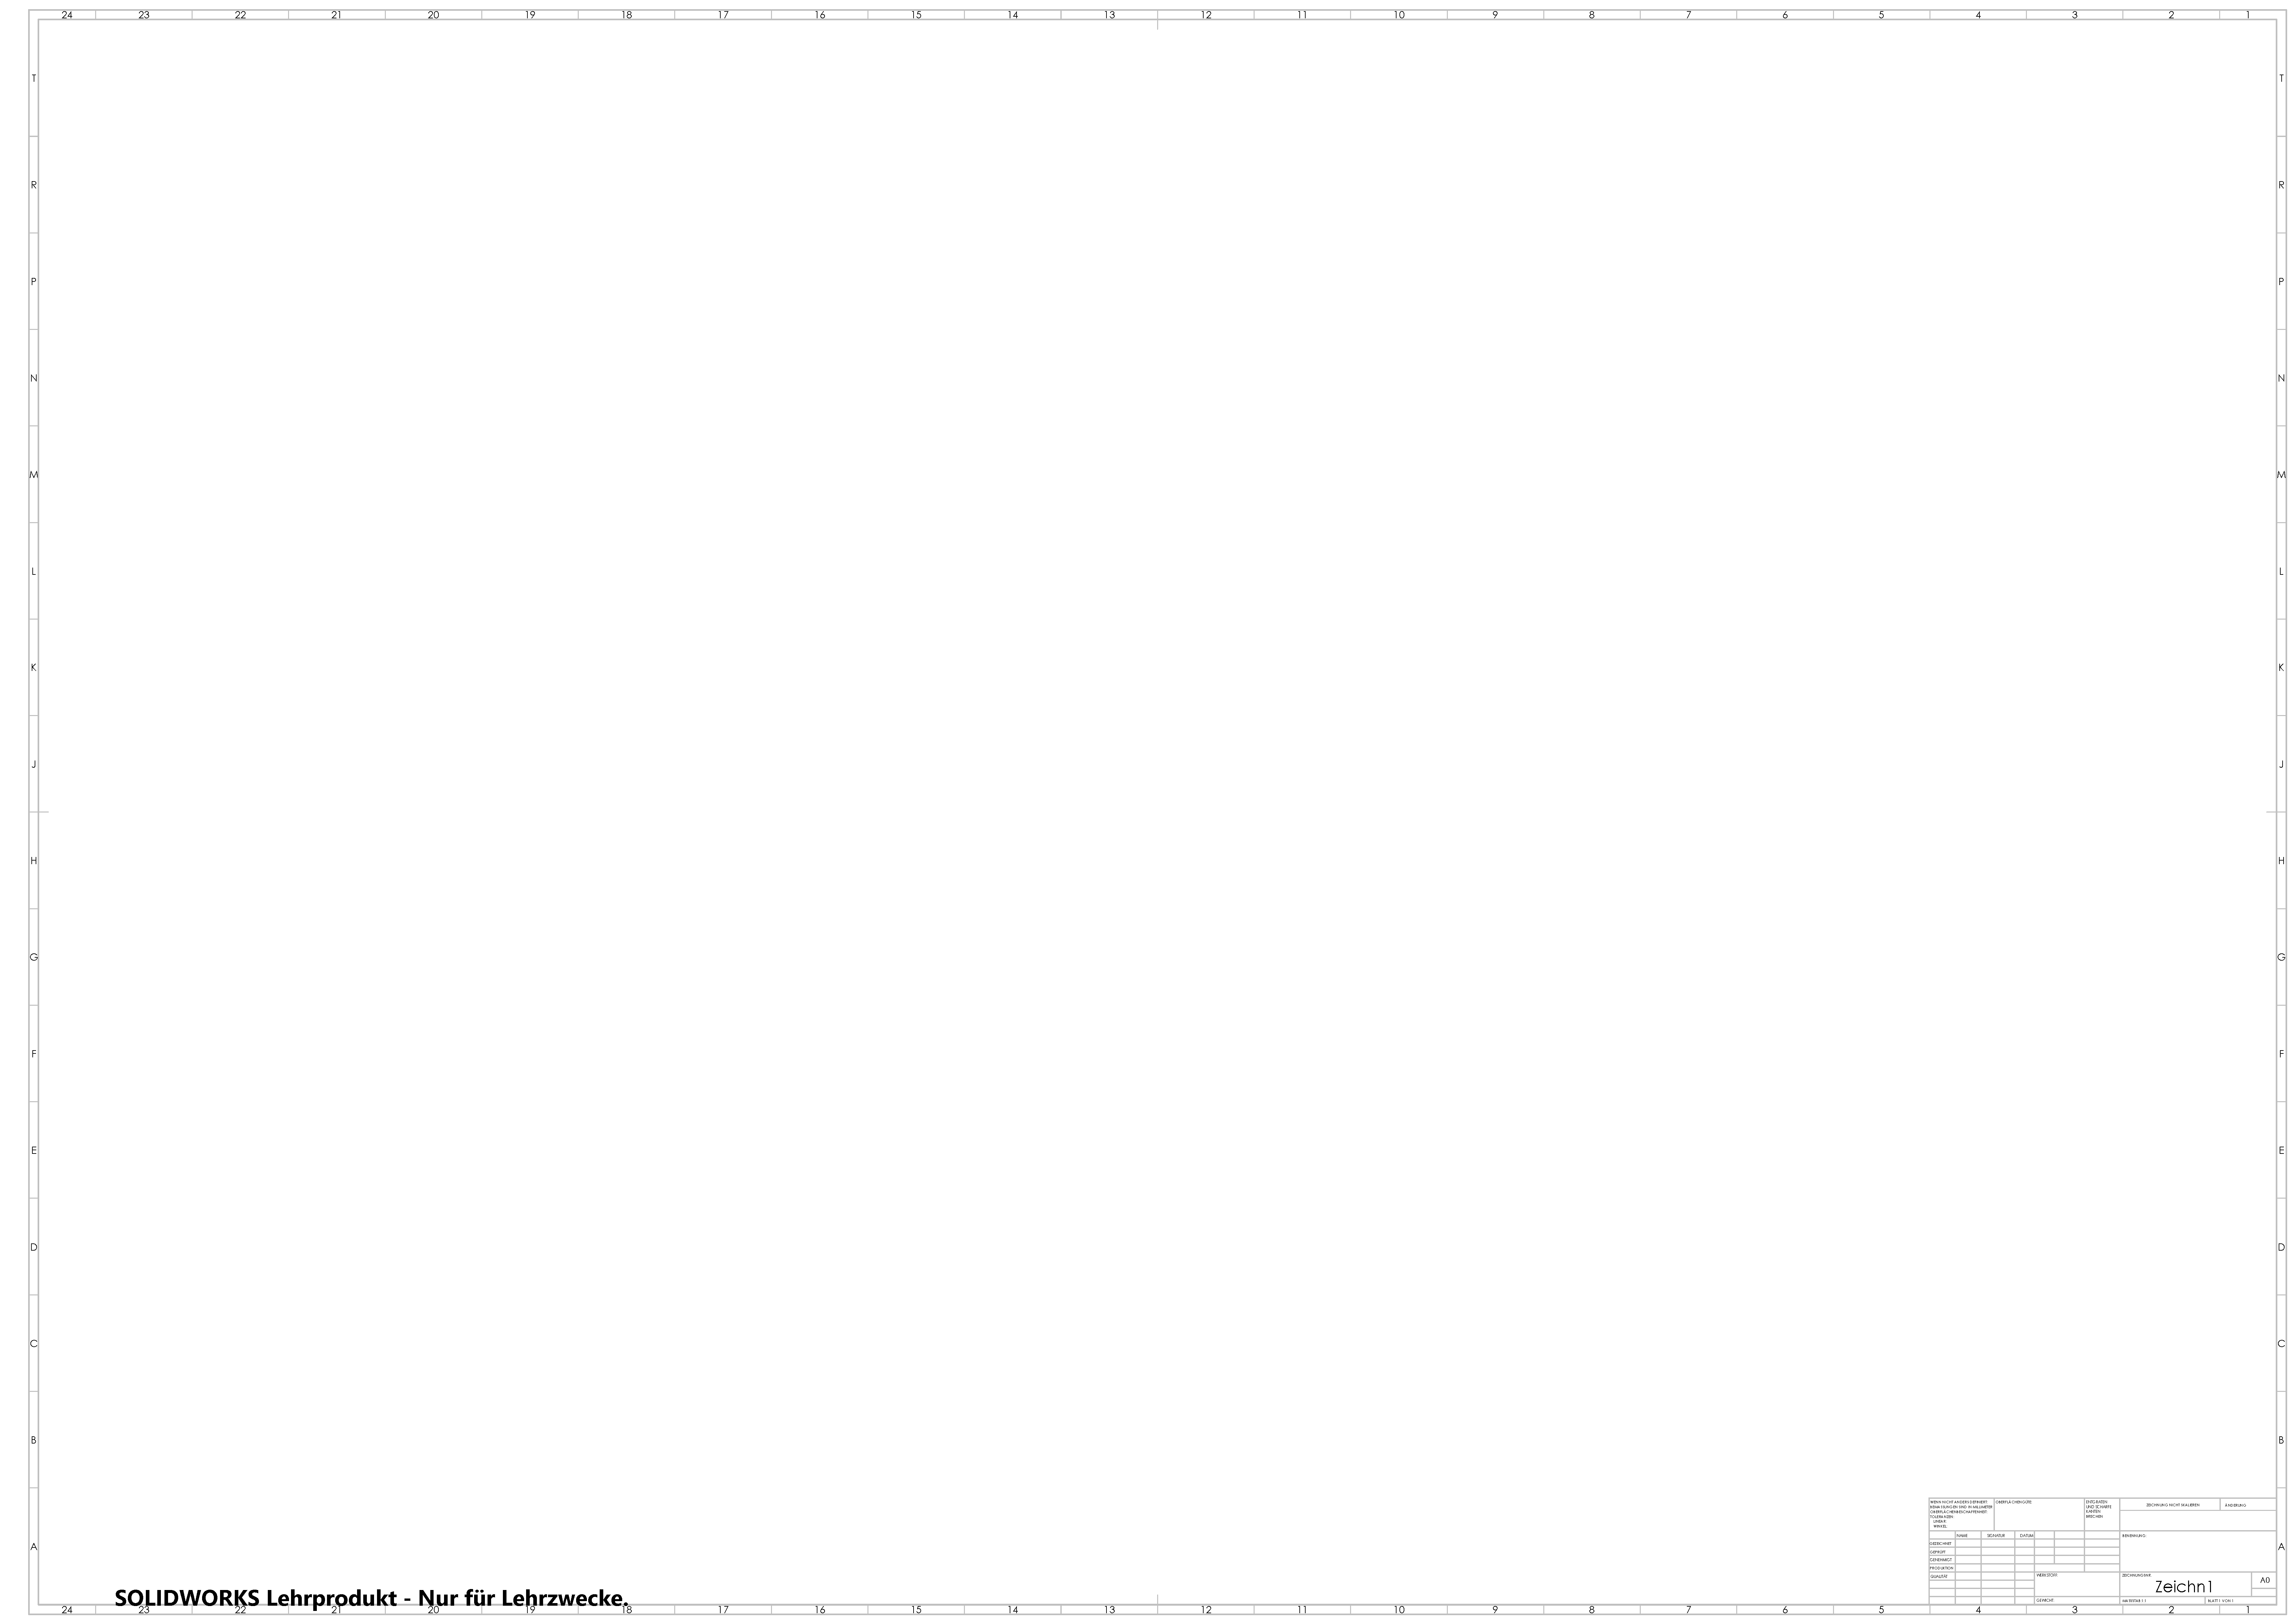
\includegraphics[width=\linewidth]{texfiles/mech/eimg/propulsion/spaceholder_technical_drawing}
    \caption{Technical Drawing}
    \label{fig:TD Motorshaft}
  \end{subfigure}
  \caption{Motor Bracket}
  \label{fig:Motorshaft}
  \end{figure}


The wheel shafts provide the mounting point for the wheels. This is done by means of a bolt circle on a flange to ensure easy mounting and, if necessary, changing of the wheels. In this shaft, the 200 Nm torque (pink) applied to the keyway is transmitted to the wheel over the entire surface of the flange. The centrifugal force (blue) is also generated again due to the 3000 rpm and this shaft is also mounted on bearings (orange) within the knuckles. You can find out more about this bearing in the suspension section. However, this shaft must be able to withstand the mass inertia of the wheel (red). This is calculated by
\(5/2 \times m_{\text{wheel}} \times a\)

\begin{figure}[ht]
\centering
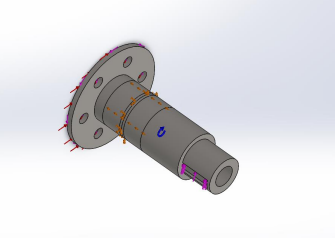
\includegraphics[width=0.6\textwidth]{texfiles/mech/eimg/propulsion/picture_forces_wheelshaft}
\caption{Forces acting on the wheelshaft}
\label{fig:wheelshaft_forces}
\end{figure}

\subsubsection{Wheels}
\begin{figure}[ht!]
  \centering
  \begin{subfigure}{.5\textwidth}
    \centering
    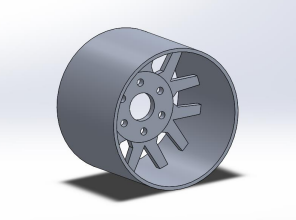
\includegraphics[width=\linewidth]{texfiles/mech/eimg/propulsion/picture_wheel}
    \caption{CAD Render}
    \label{fig:CAD Motorshaft}
  \end{subfigure}%
  \begin{subfigure}{.5\textwidth}
    \centering
    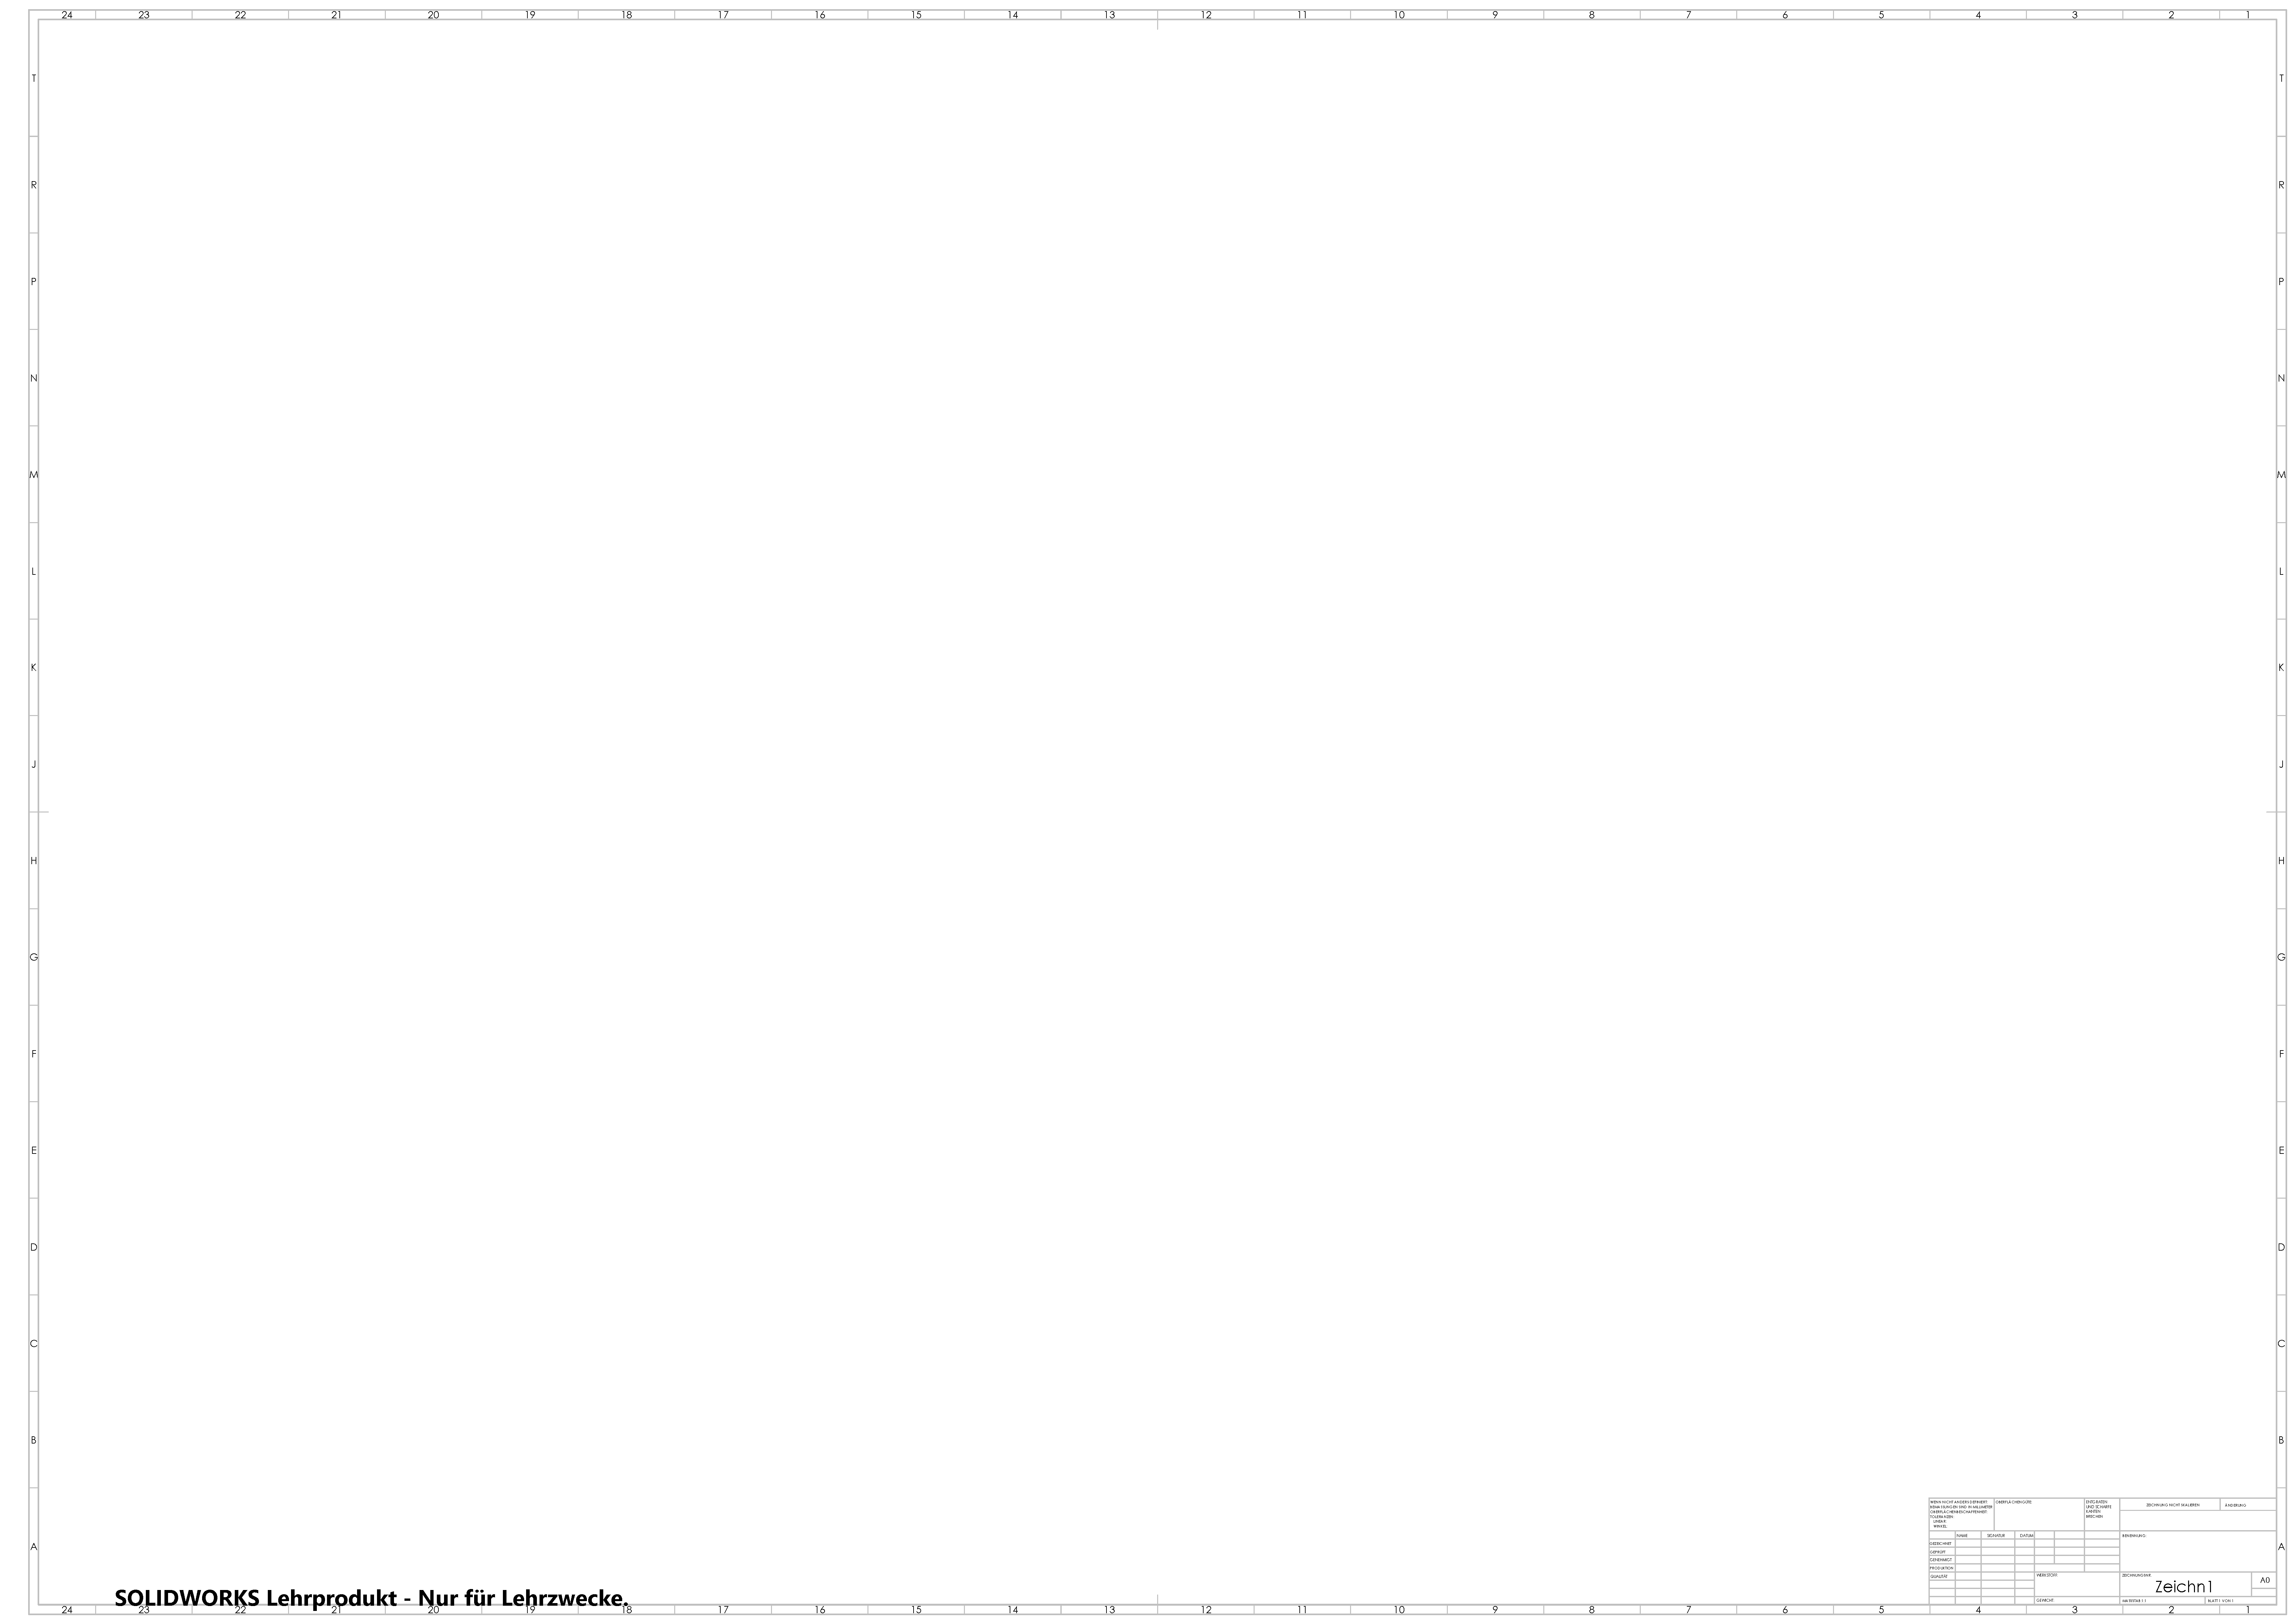
\includegraphics[width=\linewidth]{texfiles/mech/eimg/propulsion/spaceholder_technical_drawing}
    \caption{Technical Drawing}
    \label{fig:TD Motorshaft}
  \end{subfigure}
  \caption{Motor Bracket}
  \label{fig:Motorshaft}
 
\end{figure}

Finally, we transfer the torque (pink) to the wheels via the contact surface of the flange (green). The mass inertia of the wheel (red)
\(5/2 \times m_{\text{wheel}} \times a\)
, again the centrifugal force at 3000 rpm (blue) and the local pod weight of approximately 600 N (orange) also have an effect here. This weight, together with the rolling friction coefficient of the rubber cover, enables slip-free propulsion. We get this coefficient of 0,5099 by the formula
\[
\frac{m \cdot a}{m \cdot g}
\]

\begin{figure}[H]
\centering
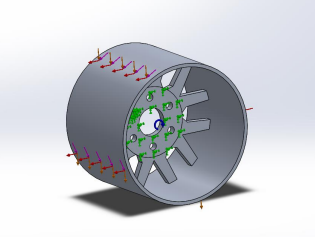
\includegraphics[width=0.6\textwidth]{texfiles/mech/eimg/propulsion/picture_forces_wheel}
\caption{Forces acting on the wheels}
\label{fig:wheel_forces}
\end{figure}


\subsubsection{Motorbracket}

\begin{figure}[ht!]
  \centering
  \begin{subfigure}{.5\textwidth}
    \centering
    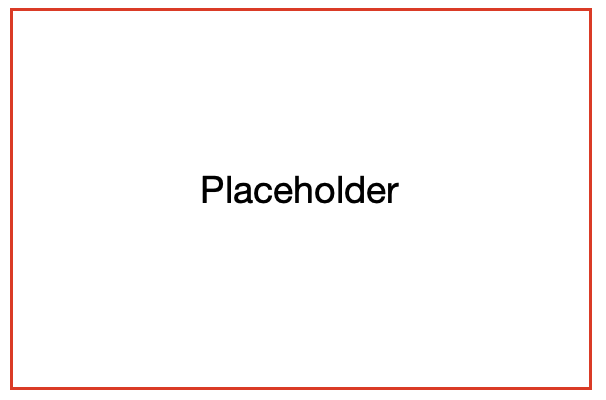
\includegraphics[width=\linewidth]{texfiles/mech/eimg/propulsion/placeholder}
    \caption{CAD Render}
    \label{fig:CAD Motorbracket}
  \end{subfigure}%
  \begin{subfigure}{.5\textwidth}
    \centering
    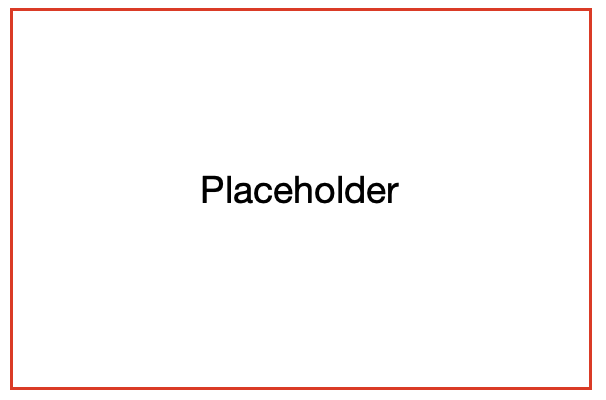
\includegraphics[width=\linewidth]{texfiles/mech/eimg/propulsion/placeholder}
    \caption{Technical Drawing}
    \label{fig:TD Motorbracket}
  \end{subfigure}
  \caption{Motor Bracket}
  \label{fig:Motorbracket}
\end{figure}

Our motor is mounted in the chassis using a bracket. This contains all the holes for screws and other components that protrude to the rear. End plates with screw holes are welded to four arms to finally screw () them into the chassis. The torque () and the inertia of the motor () prevail at this bracket.

\begin{figure}[H]
\centering
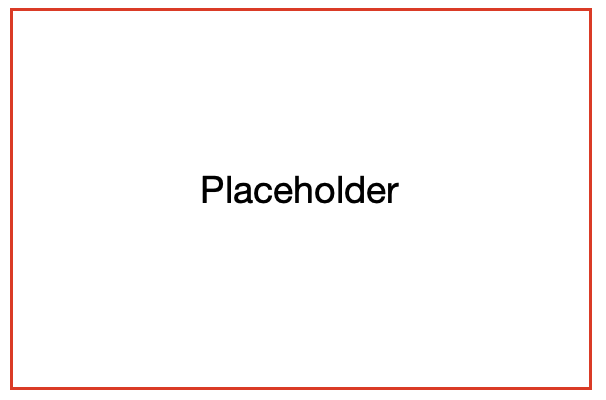
\includegraphics[width=0.6\textwidth]{texfiles/mech/eimg/propulsion/placeholder}
\caption{Forces acting on the motorbracket}
\label{fig:motorbracket_forces}
\end{figure}

\subsubsection{Motorshaftbracket}
\begin{figure}[H]
\centering
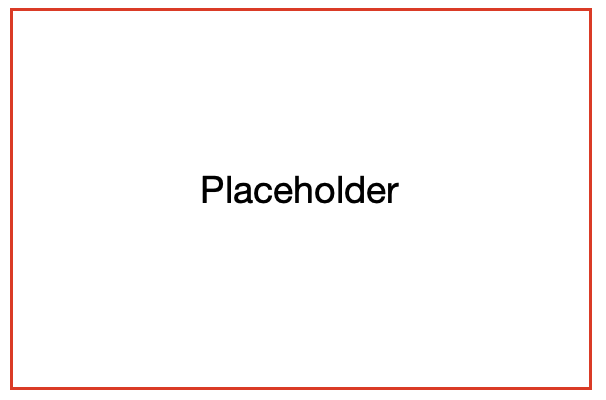
\includegraphics[width=0.6\textwidth]{texfiles/mech/eimg/propulsion/placeholder}
\caption{}
\label{}
\end{figure}

\begin{figure}[H]
\centering
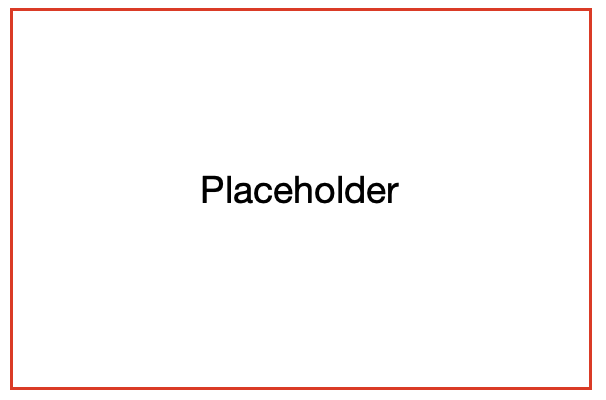
\includegraphics[width=0.6\textwidth]{texfiles/mech/eimg/propulsion/placeholder}
\caption{}
\label{}
\end{figure}

To finally support this first area of the drive system, we also support the shaft that protrudes from the motor. This is done using the CHDF35 flangebearing from Misumi. This bearing is finally integrated into the chassis by another bracket. Only the weight of the motor shaft (), its mass inertia and the wheight of the flangebearing () act on this bracket.

%\begin{figure}[H]
%\centering
%\includegraphics[width=0.6\textwidth]{texfiles/mech/eimg/propulsion/picture_forces_motorshaftbracket}
%\caption{Forces acting on the motorshaftbracket}
%\label{fig:motorshaftbracket_forces}
%\end{figure}

\subsubsection{Bearinghouse}
%\begin{figure}[H]
%\centering
%\includegraphics[width=0.6\textwidth]{texfiles/mech/eimg/propulsion/picture_bearinghouse}
%\caption{}
%\label{}
%\end{figure}

%\begin{figure}[H]
%\centering
%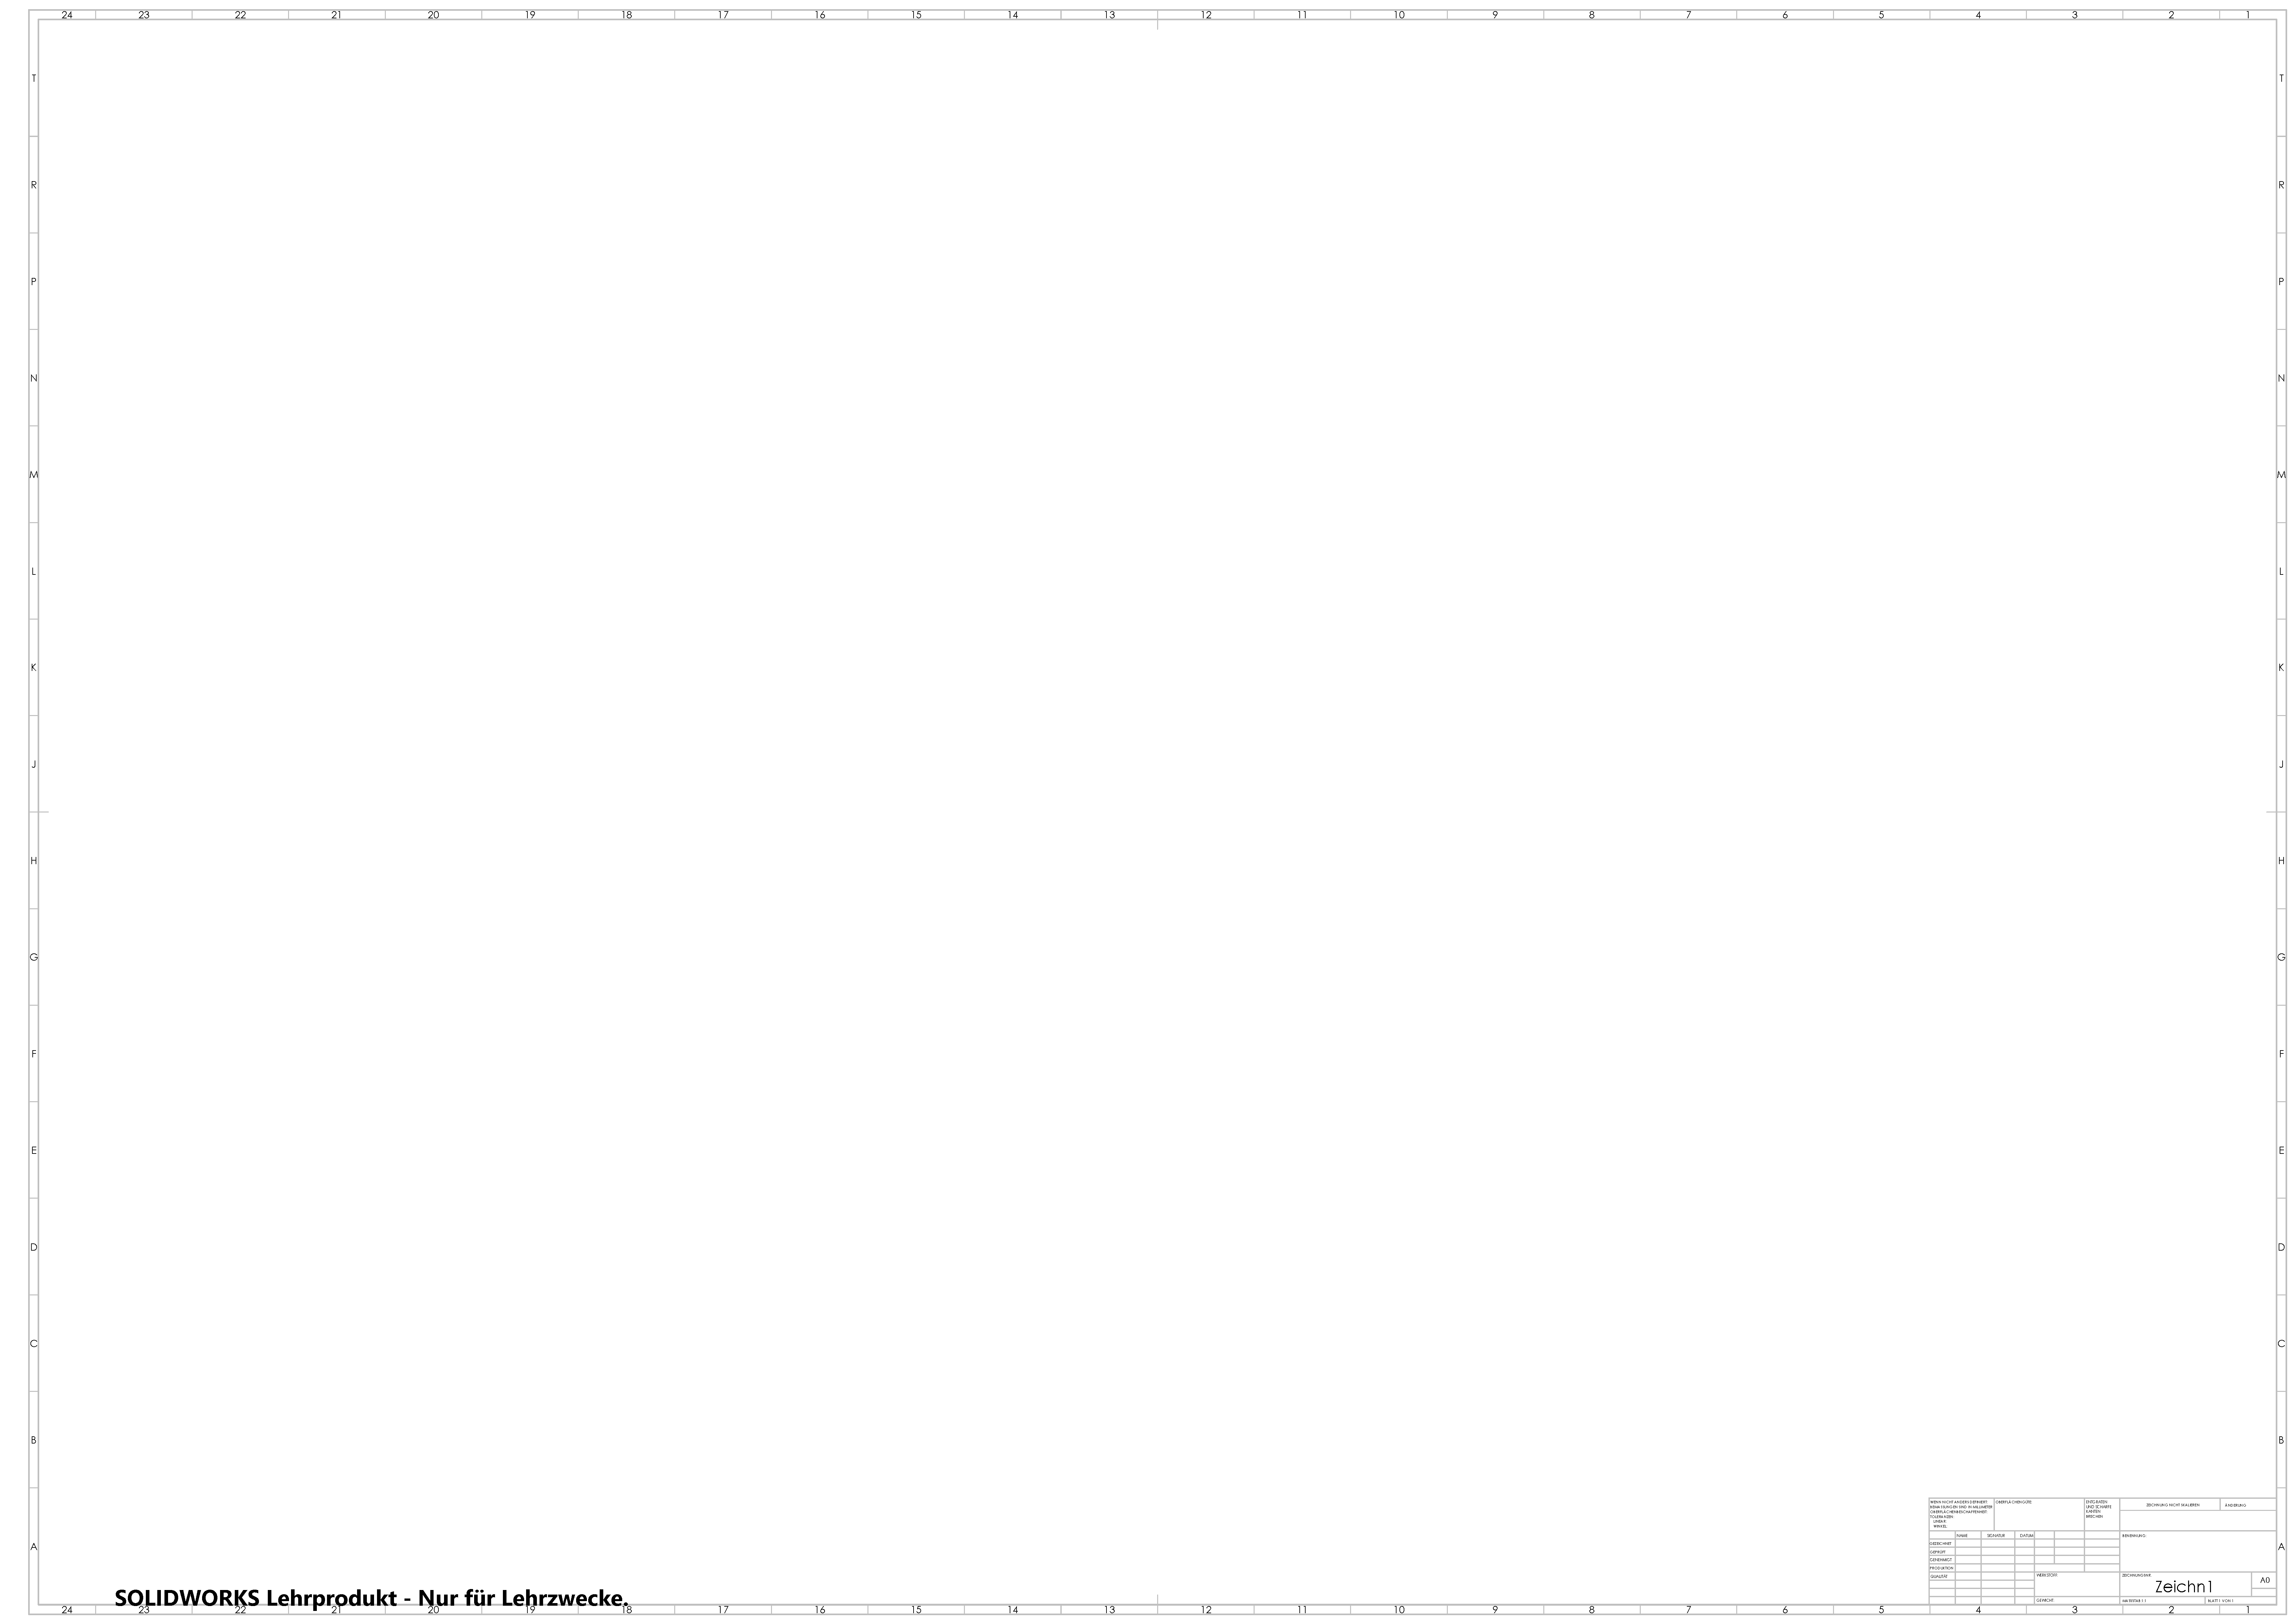
\includegraphics[width=0.6\textwidth]{texfiles/mech/eimg/propulsion/spaceholder_technical_drawing}
%\caption{}
%\label{}
%\end{figure}

To provide sufficient support for the drive axle, we mount it at two points. For space reasons, we designed the bearinghouse ourselves. The weight of the axle (pink) acts on this bearinghouse at the respective point, as well as its mass moment of inertia (). This bearing shell is installed with screws (green) on another bracket in the chassis.

%\begin{figure}[H]
%\centering
%\includegraphics[width=0.6\textwidth]{texfiles/mech/eimg/propulsion/picture_forces_bearinghouse}
%\caption{Forces acting on the bearinghouses}
%\label{fig:bearinghouse_forces}
%\end{figure}


\subsubsection{Bearingbracket}
%\begin{figure}[H]
%\centering
%\includegraphics[width=0.6\textwidth]{texfiles/mech/eimg/propulsion/picture_bearingbracket}
%\caption{}
%\label{}
%\end{figure}

%\begin{figure}[H]
%\centering
%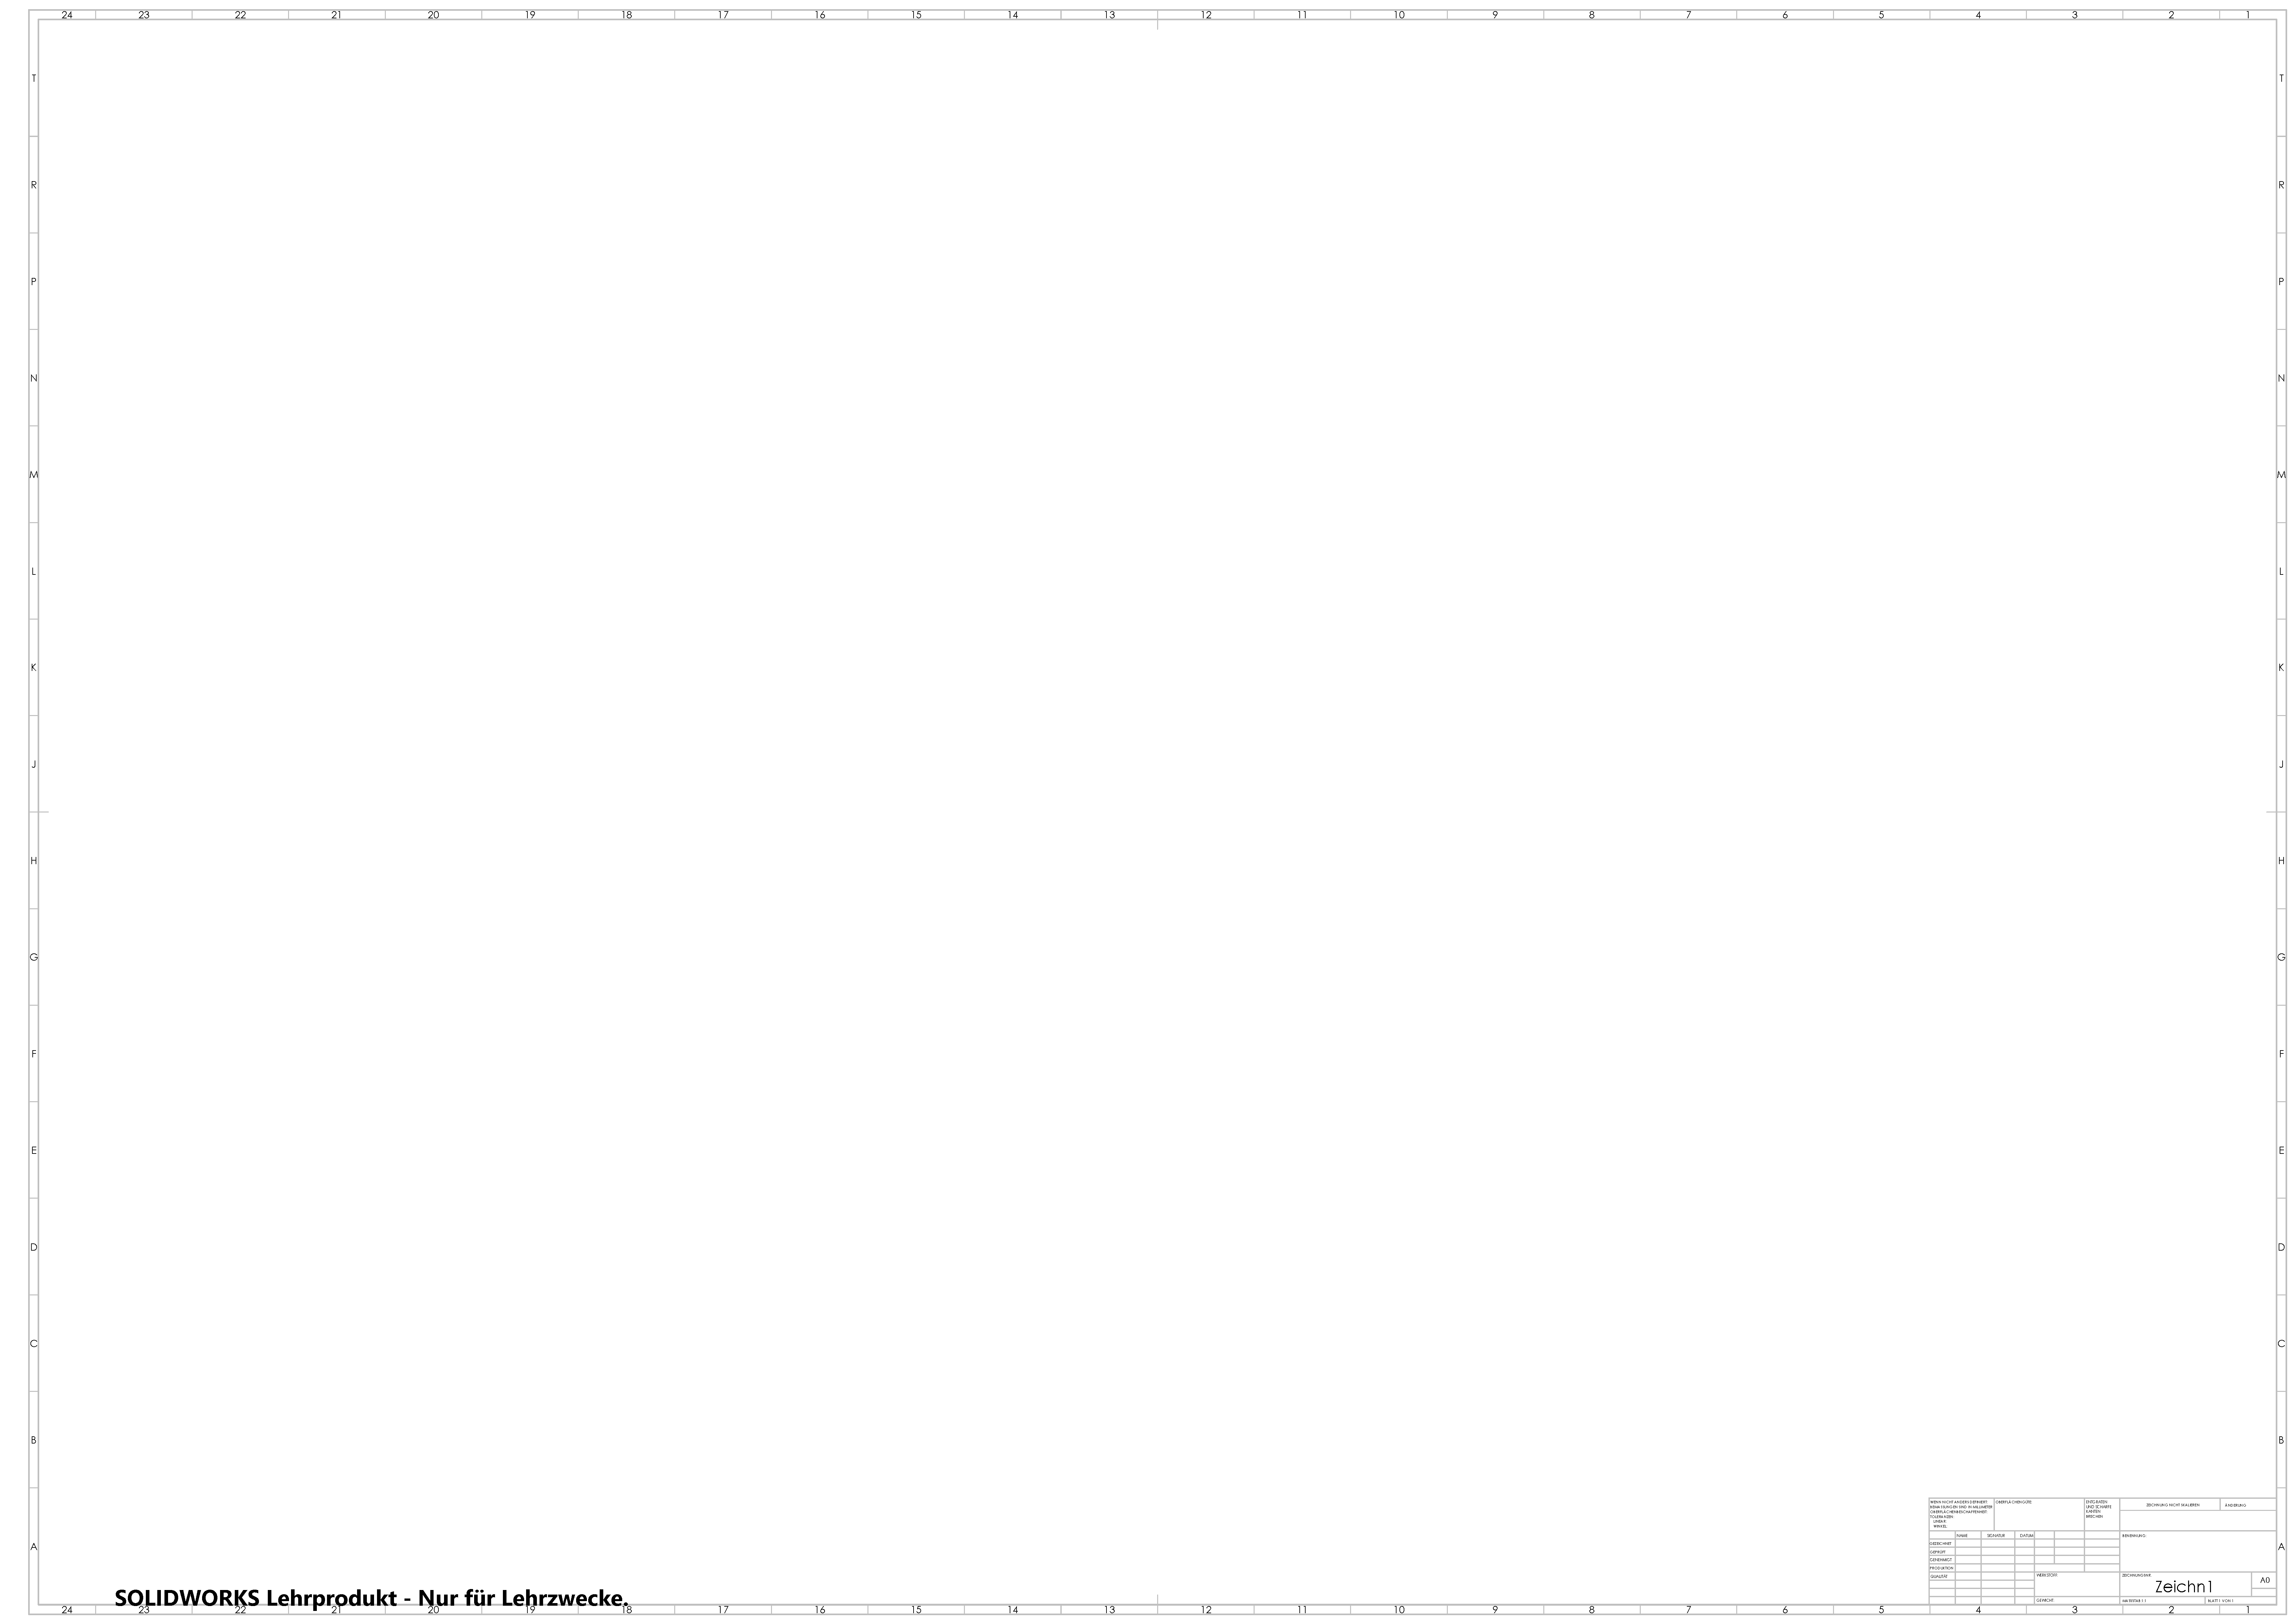
\includegraphics[width=0.6\textwidth]{texfiles/mech/eimg/propulsion/spaceholder_technical_drawing}
%\caption{}
%\label{}
%\end{figure}

As already mentioned, the bearinghouses are mounted on additional brackets. Like the motor brackets, these brackets consist of a plate with screw holes () to which end plates are welded via which the component is installed in the chassis (). The same forces act on this bracket as on the bearinghouse with the weight of the bearinghouse itself ().

%\begin{figure}[H]
%\centering
%\includegraphics[width=0.6\textwidth]{texfiles/mech/eimg/propulsion/picture_forces_bearingbracket}
%\caption{Forces acting on the bearingbrackets}
%\label{fig:bearingbracket_forces}
%\end{figure}

\subsubsection{Materials}
\begin{table}[H]
\centering
\begin{adjustbox}{width=\textwidth}
\begin{tabular}{|>{\bfseries}m{3cm}|m{2cm}|m{2.3cm}|m{2.3cm}|m{2.5cm}|}
\hline
Component & Number & Mass [kg] & Total Mass [kg] & Material \\
\hline
Motor & x1 & 7 & 14 & \\
\hline
Motorshaft & x1 & 0.4 & 0.4 & C45 Steel \\
\hline
Bevelgear z=20 & x1 & 3 & 3 & C45 Steel \\
\hline
Bevelgear z=40 & x1 & 9.6 & 9.6 & C45 Steel \\
\hline
Gearshaft Pressfitted & x1 & 0.3 & 0.3 & C45 Steel \\
\hline
Gearshaft bolted & x1 & 0.7 & 0.7 & C45 Steel \\
\hline
Shaft Joint & x2 & 4.1 & 8.2 & C45 Steel \\
\hline
Wheelshaft & x2 & 0.7 & 1.4 & C45 Steel \\
\hline
Wheel & x2 & 1.7 & 3.4 & Aluminum 6061 \\
\hline
Motorbracket & x1 &  &  & Aluminum 6061 \\
\hline
Motorshaft- bracket and flangebearing & x1 &  &  & Aluminum 6061 \\
\hline
Bearinghouse & x2 &  &  & Aluminum 6061 \\
\hline
Bearingbracket & x2 &  &  & Aluminum 6061 \\
\hline
\end{tabular}
\end{adjustbox}
\caption{Mass and Materials}
\label{table:Materials}
\end{table}

\subsubsection{FEM Results}
The result of simulating the motorshaft gives a maximum stress of \(120.1 \, \text{MN/m}^2\) and thus a safety factor of \(5.165\) and is therefore stable enough for its area of application.

\begin{figure}[H]
\centering
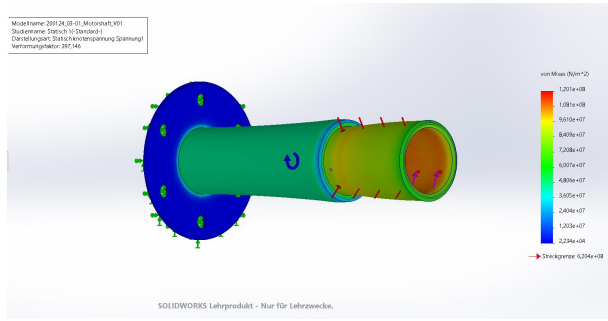
\includegraphics[width=0.6\textwidth]{texfiles/mech/eimg/propulsion/picture_simulation_motorshaft}
\caption{Finite Element Method (FEM) simulation results for the Motor shaft}
\label{fig:motorshaft_simulation}
\end{figure}

The result of simulating the pressfitted gearshaft gives a maximum stress of \(286.1 \, \text{MN/m}^2\) and thus a safety factor of \(2.027\) and is therefore stable enough for its area of application.

\begin{figure}[H]
\centering
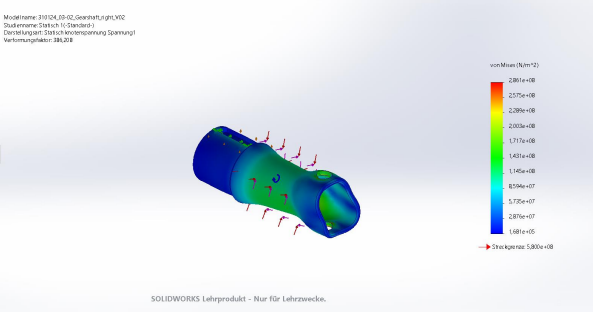
\includegraphics[width=0.6\textwidth]{texfiles/mech/eimg/propulsion/picture_simulation_gearshaft_right}
\caption{Finite Element Method (FEM) simulation results for the pressfitted Gearshaft}
\label{fig:gearshaft_simulation}
\end{figure}

The result of simulating the bolted gearshaft gives a maximum stress of \(288.1 \, \text{MN/m}^2\) and thus a safety factor of \(2.013\) and is therefore stable enough for its area of application.

\begin{figure}[H]
\centering
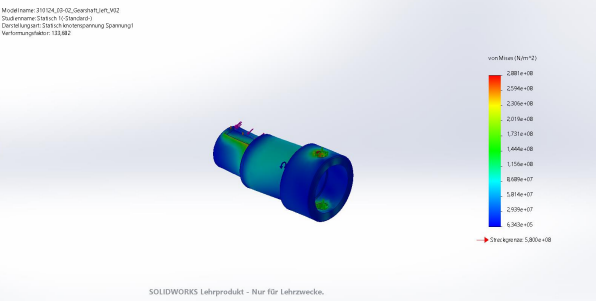
\includegraphics[width=0.6\textwidth]{texfiles/mech/eimg/propulsion/picture_simulation_gearshaft_left}
\caption{Finite Element Method (FEM) simulation results for the bolted Gearshaft}
\label{fig:gearshaft_simulation}
\end{figure}

The result of simulating the wheelshaft gives a maximum stress of \(284 \, \text{MN/m}^2\) and thus a safety factor of \(2.042\) and is therefore stable enough for its area of application. As this part is identical on both sides of the pod and has to withstand the same forces, we are only showing a single simulation here.

\begin{figure}[ht]
\centering
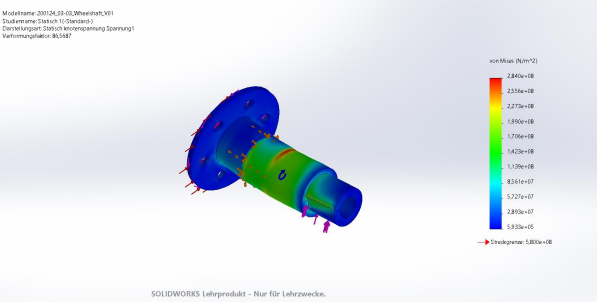
\includegraphics[width=0.6\textwidth]{texfiles/mech/eimg/propulsion/picture_simulation_wheelshaft}
\caption{Finite Element Method (FEM) simulation results for the wheelshaft}
\label{fig:wheelshaft_simulation}
\end{figure}

The result of simulating the wheel gives a maximum stress of \(19.89 \, \text{MN/m}^2\) and while we manufacture this of a Aluminum 6061 compuond, a safety factor of \(2.772\) and is therefore stable enough for its area of application. As this part is identical on both sides of the pod and has to withstand the same forces, we are only showing a single simulation here.

\begin{figure}[H]
\centering
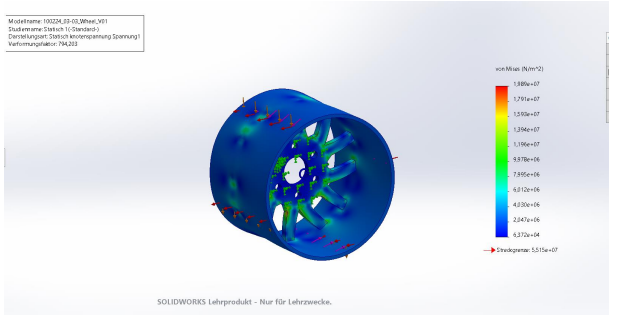
\includegraphics[width=0.6\textwidth]{texfiles/mech/eimg/propulsion/picture_simulation_wheel}
\caption{Finite Element Method (FEM) simulation results for the wheels}
\label{fig:wheel_simulation}
\end{figure}

The result of simulating the motorbracket gives a maximum stress of \(XX \, \text{N/m}^2\) and thus a safety factor of \(XX\) and is therefore stable enough for its area of application. As this part is identical on both sides of the pod and has to withstand the same forces, we are only showing a single simulation here.

%\begin{figure}[H]
%\centering
%\includegraphics[width=0.6\textwidth]{texfiles/mech/eimg/propulsion/picture_simulation_motorbracket}
%\caption{Finite Element Method (FEM) simulation results for the motorbracket}
%\label{fig:motorbracket_simulation}
%\end{figure}

The result of simulating the motorshaftbracket gives a maximum stress of \(XX \, \text{N/m}^2\) and thus a safety factor of \(XX\) and is therefore stable enough for its area of application. As this part is identical on both sides of the pod and has to withstand the same forces, we are only showing a single simulation here.

%\begin{figure}[H]
%\centering
%\includegraphics[width=0.6\textwidth]{texfiles/mech/eimg/propulsion/picture_simulation_motorshaftbracket}
%\caption{Finite Element Method (FEM) simulation results for the motorshaftbracket}
%\label{fig:motorshaftbracket_simulation}
%\end{figure}

The result of simulating the bearinghouse gives a maximum stress of \(XX \, \text{N/m}^2\) and thus a safety factor of \(XX\) and is therefore stable enough for its area of application. As this part is identical on both sides of the pod and has to withstand the same forces, we are only showing a single simulation here. As this part is identical on both sides of the pod and has to withstand the same forces, we are only showing a single simulation here.

%\begin{figure}[H]
%\centering
%\includegraphics[width=0.6\textwidth]{texfiles/mech/eimg/propulsion/picture_simulation_bearinghouse}
%\caption{Finite Element Method (FEM) simulation results for the bearinghouses}
%\label{fig:bearinghouse_simulation}
%\end{figure}

The result of simulating the bearingbracket gives a maximum stress of \(XX \, \text{N/m}^2\) and thus a safety factor of \(XX\) and is therefore stable enough for its area of application. As this part is identical on both sides of the pod and has to withstand the same forces, we are only showing a single simulation here. As this part is identical on both sides of the pod and has to withstand the same forces, we are only showing a single simulation here.

%\begin{figure}[H]
%\centering
%\includegraphics[width=0.6\textwidth]{texfiles/mech/eimg/propulsion/picture_simulation_bearingbracket}
%\caption{Finite Element Method (FEM) simulation results for the bearingbrackets}
%\label{fig:bearingbracket_simulation}
%\end{figure}

\subsubsection{Mesh and Boundary Conditions}
For meshing and specify all required parameters for a successful simulation, we used the standardsettings of Solidworks.

\subsection{Control section}
Control architecture: The pod only uses a Permanent Magnet Synchronous Motor (PMSM) to move. The traction inverter that we use transforms DC power from the batteries to AC 3-phase power in the motor. Due to the device we use being an OEM product, we cannot give information about the underlying control theory, besides of that it uses field-oriented control. \\
Our motor is equipped with a resolver measuring the rotor position and speed, the Tamagawa TS2620N21E11 Brushless Pancake resolver which outputs to the inverter. It also has a temperature sensor.
The interface with the electric system is both physical and informational, through the HV line and the CAN Bus, respectively, with the inverter acting as the coordinating device, having power and data inputs. 
\begin{figure}[H]
  \centering
  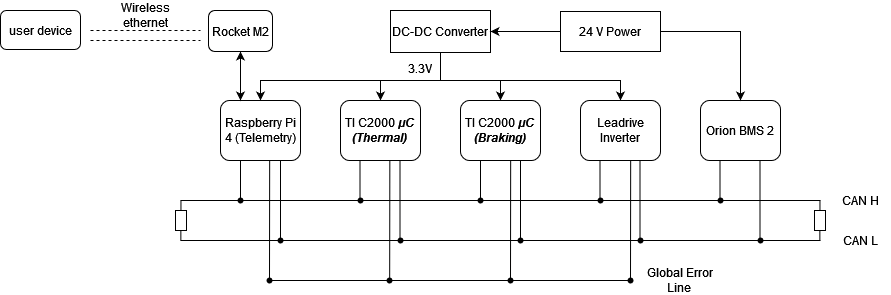
\includegraphics[width=0.8\textwidth]{texfiles/mech/eimg/propulsion/telemetrysystems}
  \caption{CAN Bus}
  \label{fig:canbus}
\end{figure}
Our inverter is connected to the LV power source for control and to the HV power source for the motor. It has 
several control inputs to start, or end operating.
All of the commands, especially the ones of the user, are processed over CAN. We have the option to either 
control speed, or torque, while setting a speed, torque, and current maximum limit. We decided to use the speed control only for ensuring additional safety in case of electronics failure. The current limit is set according to the current limit of the motor. \\
The inverter, used for automotive applications, is rated for ASIL-C level according to ISO 26262, after
adapting it to our target application by setting up the inverter correctly with the specifications of our motor. \\
The inverter is able to give negative torque, which enables regenerative braking. However, due to our technical constraints this year, and the short length of track, we decided not to implement this feature, while we are fully Acknowledging that regenerative braking significantly helps to reduce the energy consumption, as experiences from the railway sector have shown, along with an efficient U-shaped tunnel design around stations, decelerating through an ascent before stations, and further accelerating through a slight descent after stations \footnote{These tunnel construction methods are not part of the research work of the team working on traction systems.}. \\
Our procedure at EHW will consist of \begin{itemize}
  \item Setup/Initialize
  \item Accelerating
  \item (Cruising)
  \item Braking
  \item Shutoff
\end{itemize}
We will not decelerate through the traction system, but through our friction brakes.

\subsection{Manufacturing Process}
\begin{table}[H]
\centering
\begin{adjustbox}{width=\textwidth}
\begin{tabular}{|>{\bfseries}m{5cm}|m{1,5cm}|m{8cm}|}
\hline
Component & Number & Required procedures \\
\hline
Motorshaft & x1 & latheturning, milling \\
\hline
Gearshaft Pressfitted & x1 & latheturning, milling, hydraulic pressing \\
\hline
Gearshaft bolted & x1 & latheturning, milling \\
\hline
Wheelshaft & x2 & latheturning, milling \\
\hline
Wheel & x2 & latheturning, milling \\
\hline
Motorbracket & x1 & lasercutting  \\
\hline
Wheelshaftbracket & x1 & lasercutting  \\
\hline
Bearinghouse & x2 & lasercutting  \\
\hline
Bearingbracket & x2 & lasercutting, welding \\
\hline
\end{tabular}
\end{adjustbox}
\caption{Components and Manufacturing Details}
\label{table:components}
\end{table}

\subsection{Integration process}

At Yash: Please add information here.

\subsubsection{Assembling}
Describe how the parts will be assembled, including integration into subordinate structures/systems if applicable.

\subsubsection{Assembly interaction}
If applicable, describe how the assembly interacts with other assemblies.



\subsection{Safety considerations }
(a) Discuss the safety factor applied to structural elements. \\
(b) If applicable, discuss the safety factor applied to the demagnetization of permanent mag-
nets.\\
(c) If applicable, discuss high voltage safety considerations for the motor.\\
(d) Discuss worst-case scenarios (e.g., worst-case braking deceleration) and what you plan
to do to avoid or contain them.\\

\subsection{FMEA}
\textbf{WILL BE DONE BY PM}

\subsubsection{Expected Outcomes}
Detail the anticipated results from the testing and validation processes.

\subsubsection{Risk Mitigation}
Discuss the potential risks associated with the system and how they will be mitigated.

\paragraph{Impact Resistance}
Detail a contingency plan in case the system does not perform as expected.


\subsection{Testing}
Provide a test plan including setup, procedure, and expected outcomes.
Outline which factors are critical to success and how they will be validated.
\subsubsection{Preliminary Inverter Safety and Testing Plan}
Based on the datasheet provided by our Traction Inverter supplier (LEADRIVE Technology Germany GmbH), the inverter is a ASIL-C compatible device. Therefore, it already internally consists both hardware and software safety features to protect both the power electronics and the motor such as the Overvoltage, Over Current and Motor temperature. However, in the interest of ensuring electrical safety of both the pod and the team members the following tests will be performed:

\begin{table}[H]
    \centering
    \begin{adjustbox}{width=\textwidth}
    \begin{tabular}{|p{7.5cm}|p{10cm}|}
        \hline
        \textbf{Parameter} & \textbf{Test Method} \\
        \hline
        Over Voltage & Set the over voltage threshold in the inverter to a low voltage to see if the over voltage error is thrown and verify the PWM Phase outputs using Oscilloscope to confirm that the inverter is disabled, thereby verifying the functionality.\\
	\hline
	Over Current & Set the over current threshold in the inverter to a low current and drive the motor to trigger an over current fault, verify the PWM Phase outputs using Oscilloscope to confirm that the inverter is disabled, thereby verifying the functionality.\\
	\hline
	Motor Over Temperature &  Simulate an overtemperature by selecting an appropriate resistance as a substitute to the Thermistor inputs and verify the error status of the inverter thereby verifying the functionality.\\
	\hline
	Inverter Over Temperature & Functionality cannot be verified independantly as the thresholds are set by the manufacturer for the internal hardware.\\
         \hline
	Emergency Shutdown & Simulate an global error by pulling the global error connector to a low state by connecting to ground, verify the error status via CAN and verify the PWM phase outputs using Oscilloscope to confirm that the inverter is disabled.\\
	\hline
    \end{tabular}
    \end{adjustbox}
    \label{tab:preliminvtest}
    \caption{List of Preliminary Inverter Tests}
    
\end{table}

\noindent
The adjustments of the thresolds/calibration data mentioned in the table \ref{tab:preliminvtest} is performed using XCP via CAN based on the manufacturer's recommendations.
\subsection{Full-scale adaptation}
\begin{itemize}
  \item Functions like a conventional railway system
  \item Full-scale acceleration is possible
  \item The inverter is designed for the dimensions of an electric car
  \item Once the pod starts levitating, the wheels are lifted, and the current friction-based propulsion system is deactivated
  \item Levitation on two guides is also built in the real world \footnote{https://www.maglevboard.net/en/visuals/photos/271-linimo-urban-maglev-cn}
\end{itemize}

\subsection{References}

\begin{figure}[H]
\centering
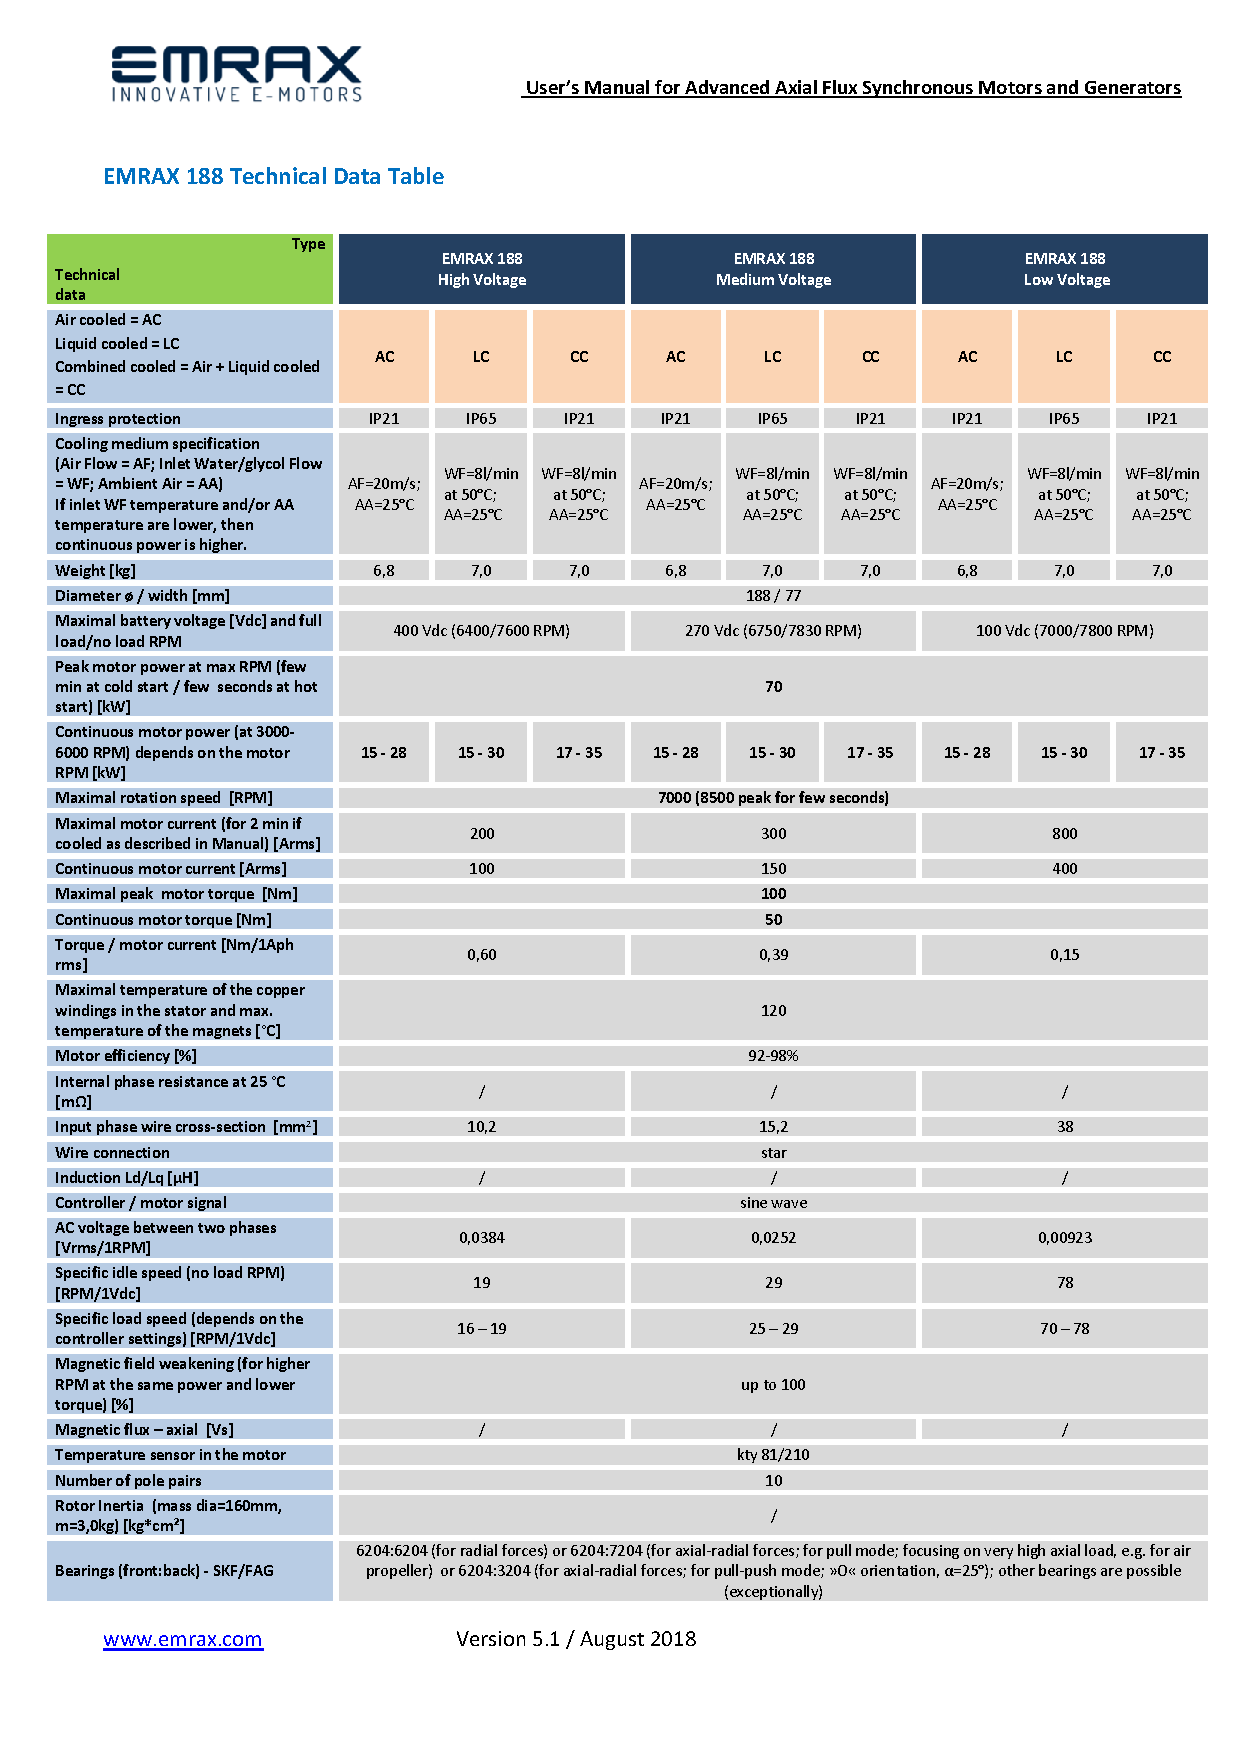
\includegraphics[width=0.9\textwidth]{texfiles/mech/eimg/propulsion/table_motor}
\caption{Motor Specifications}
\label{tab: Motor Specifications}
\end{figure}
 \newpage
